\chapter{最优体积约束比}
针对体积约束比结果不准确和LBB稳定性条件验证过程复杂的问题,本章采用泛函分析的手段,验证LBB稳定性条件与特征值问题的等价性。
详细讨论特征值问题非零特征值个数与体积约束比之间的联系,从而建立体积约束比和LBB稳定性条件之间的关系。
以此,构建考虑体积约束比的新型LBB稳定系数估计表达式,从而确定最优体积约束比。

\section{LBB稳定性条件与特征值问题}

基于LBB稳定性条件\eqref{ch:2:eq:LBB},假设$\mathcal P_h:V_h \rightarrow Q_h$ 是$\mathcal P$的正交投影算子,定义为:
\begin{equation}\label{ch_3:eq:Ph}
    b(q_h,\boldsymbol v_h) = (q_h, \mathcal P \boldsymbol v_h) = (q_h, \mathcal P_h \boldsymbol v_h), \quad \forall q_h \in Q_h
\end{equation}
式中散度算子$\mathcal P:V\rightarrow Q$。于是,LBB稳定性条件\eqref{ch:2:eq:LBB}可以改写为:
\begin{equation} \label{ch_3:eq:r11}
    \beta \le \inf_{q_h \in Q_h} \sup_{\boldsymbol v_h \in V_h} \frac{\vert b(q_h,\boldsymbol v_h) \vert}{\Vert q_h \Vert_Q \Vert \boldsymbol v_h \Vert_V} 
    \le \inf_{q_h \in Q_h} \sup_{\boldsymbol v_h \in V_h} \frac{\vert (q_h,\mathcal P_h \boldsymbol v_h) \vert}{\Vert q_h \Vert_Q \Vert \boldsymbol v_h \Vert_V}
\end{equation}

式\eqref{ch_3:eq:r11}对于任意的$q_h \in Q_h$均成立,可知其对于所有的$Q_h$均成立,又有$\mathcal P_h$的相空间$\mathrm{Im}\mathcal P_h \in Q_h$。因此,对于$q_h \in \mathrm{Im}\mathcal P_h$也应成立。LBB稳定性条件可以进一步改写为:
\begin{equation} \label{ch_3:eq:r12}
        \beta \le \inf_{q_h \in Q_h} \sup_{\boldsymbol v_h \in V_h} \frac{\vert b(q_h,\boldsymbol v_h) \vert}{\Vert q_h \Vert_Q \Vert \boldsymbol v_h \Vert_V} 
        \le \inf_{q_h \in \mathrm{Im}\mathcal P_h} \sup_{\boldsymbol v_h \in V_h} \frac{\vert (q_h,\mathcal P_h \boldsymbol v_h) \vert}{\Vert q_h \Vert_Q \Vert \boldsymbol v_h \Vert_V}
\end{equation}

由相空间$\mathrm{Im}\mathcal P_h \in Q_h$,根据柯西--施瓦茨(Cauchy--Schwarz)不等式\cite{philippeg.2013},有
\begin{equation}
    \vert (q_h,\mathcal P_h \boldsymbol v_h) \vert \le \Vert q_h \Vert_Q \Vert \mathcal P_h \boldsymbol v_h \Vert_Q
\end{equation}
同时,当且仅当$q_h=\mathcal P_h \boldsymbol v_h$时,等式成立,即
\begin{equation}\label{ch_3:eq:equality}
    \vert (q_h,\mathcal P_h \boldsymbol v_h) \vert = \Vert q_h \Vert_Q \Vert \mathcal P_h \boldsymbol v_h \Vert_Q, \quad \forall \boldsymbol v_h \in V'_h
\end{equation}
对于给定的 $q_h\in \mathrm{Im}\mathcal P_h$,空间$V'_h$定义为:$V'_h = \{ \boldsymbol v_h \in V_h \; \vert \; \mathcal P_h \boldsymbol v_h = q_h \}$。
当等式成立时,从式\eqref{ch_3:eq:r12}可知,$q_h$和$\boldsymbol v_h$均不可以等于零。因此,空间$V'_h \subset V_h\setminus \ker P_h$,其中 $\ker \mathcal P_h \subset V$ 是 $\mathcal P_h$ 的核,定义为: $\ker \mathcal P_h = \{ \boldsymbol v \in V \;\vert\; \mathcal P_h \boldsymbol v = 0 \}$。
将式\eqref{ch_3:eq:equality}代回到式\eqref{ch_3:eq:r12}中,此时不等式\eqref{ch_3:eq:r12}的右边可以改写为:
\begin{equation}\label{ch_3:eq:r13}
    \begin{split}
    \inf_{q_h \in \mathrm{Im}\mathcal P_h}\sup_{\boldsymbol v_h\in V_h} \frac{\vert (q_h,\mathcal P_h \boldsymbol v_h) \vert}{\Vert q_h \Vert_Q \Vert \boldsymbol v_h \Vert_V} &=
    \inf_{q_h \in \mathrm{Im}\mathcal P_h}\sup_{\boldsymbol v_h\in V'_h} \frac{\vert (\Vert q_h \Vert_Q \Vert \mathcal P_h \boldsymbol v_h \Vert_Q}{\Vert q_h \Vert_Q \Vert \boldsymbol v_h \Vert_V} \\
    &=\inf_{q_h \in \mathrm{Im}\mathcal P_h}\sup_{\boldsymbol v_h\in V'_h} \frac{\Vert \mathcal P_h 
    \boldsymbol v_h \Vert_Q}{\Vert \boldsymbol v_h \Vert_V} 
    \end{split}
\end{equation}
结合式\eqref{ch_3:eq:r12}、\eqref{ch_3:eq:r13}可得LBB稳定系数估算式:
\begin{equation}\label{ch_3:eq:r1}
    \beta \le \inf_{V'_h \subset V_h \setminus \ker \mathcal P_h} \sup_{v_h \in V'_h} \frac{\Vert \mathcal P_h \boldsymbol v_h \Vert_Q}{\Vert \boldsymbol v_h \Vert_V}
\end{equation}
根据混合离散里兹–伽辽金变分方程\eqref{ch_2:eq:ritz_mix},式\eqref{ch_3:eq:r1}可以改写为:
\begin{equation}\label{ch_3:eq:r2}
    \beta \le \inf_{V'_h \subset V_h \setminus \ker \mathcal P_h} \sup_{v_h \in V'_h} \frac{\Vert\tilde{\varepsilon^v_h}\Vert_Q}{\Vert \varepsilon^d_h\Vert_V}
\end{equation}
再根据最小--最大值原理 \cite{babuska1991a}:
\begin{equation}
    \lambda_k = \min_{{V_k\subset H},{\dim V_k=k}}\max_{u\in V_k}\boldsymbol{R(u)} = \max_{u\in U_k \equiv \text{sp}(u_1,\dots,u_k)}\boldsymbol{R}(u),\quad k=1,2,\dots
\end{equation}
式\eqref{ch_3:eq:r2}可得到刚度矩阵$\boldsymbol K^v$ 和 $\boldsymbol K^d$的特征值关系\eqref{ch_2:eq:eigenvalue},即LBB稳定系数估算式\eqref{ch_3:eq:r1}计算考虑最小非零特征值。
\section{特征值问题与体积约束比}

为了进一步找出最优约束自由度数量,定义$\mathcal I_h$为有限元插值,有$V_h=\mathcal I_h V$。引入$n_u$维完备多项式空间$P_{n_u}$ , $V_{n_u}$ 是相对应的位移多项式空间,且 $V_{n_u} = P_{n_u}^{n_d}$,$V_{n_u} \subset V$的维度为$n_d\times n_u$。此时,$V_h$ 和 $V_{n_u}$的维度相同,即$\dim V_{n_u}=\dim V_h = n_d\times n_u$,有且仅有唯一的$\boldsymbol v \in V_{n_u}$ 满足$\boldsymbol v_h = \mathcal I_h \boldsymbol v$,。于是式\eqref{ch_3:eq:r1}的右边可以改写为:
\begin{equation}\label{ch_3:eq:r21}
    \inf_{V'_h \subset V_h\setminus \ker \mathcal P_h}\sup_{\boldsymbol v_h \in V_h'} \frac{\Vert \mathcal P_h \boldsymbol v_h \Vert_Q}{\Vert \boldsymbol v_h \Vert_V} = 
    \inf_{V'\subset V_{n_u}\setminus \ker \mathcal P_h \mathcal I_h}\sup_{\boldsymbol v \in V'} \frac{\Vert \mathcal P_h \mathcal I_h \boldsymbol v \Vert_Q}{\Vert \mathcal I_h \boldsymbol v \Vert_V}
\end{equation}

根据三角不等式、柯西--施瓦茨不等式和式\eqref{ch_3:eq:Ph}中的等式关系可得:
\begin{equation}\label{ch_3:eq:interpolation1}
    \begin{split}
        \Vert \mathcal P_h \mathcal I_h \boldsymbol v \Vert_Q &= 
        \sup_{q_h \in Q_h} \frac{\vert (q_h, \mathcal P_h \mathcal I_h \boldsymbol v) \vert}{\Vert q_h \Vert_Q}\quad \text{三角不等式}\\
        &=\sup_{q_h \in Q_h} \frac{\vert (q_h, \mathcal P \mathcal I_h \boldsymbol v) \vert}{\Vert q_h \Vert_Q} \quad \text{式\eqref{ch_3:eq:Ph}等式关系}\\
        &\le \sup_{q_h \in Q_h} \frac{\vert (q_h, \mathcal P \boldsymbol v)\vert + \vert (q_h, \mathcal P \boldsymbol v - \mathcal P \mathcal I_h \boldsymbol v) \vert}{\Vert q_h \Vert_Q} \quad \text{柯西--施瓦茨不等式}\\
        &= \Vert \mathcal P_h \boldsymbol v \Vert_Q
        + \Vert \mathcal P(\mathcal I - \mathcal I_h) \boldsymbol v \Vert_Q \quad \text{三角不等式}\\
    \end{split}
\end{equation}
显然,式\eqref{ch_3:eq:interpolation1}右侧的第二项和第三项是$V_h$中近似值的插值误差和正交投影误差,可以由如下式子估计\cite{yosida1995}:
\begin{equation}\label{ch_3:eq:interpolation2}
        \Vert \mathcal P(\mathcal I - \mathcal I_h) \boldsymbol v \Vert_Q \le Ch \vert \boldsymbol v \vert_{H_2} 
\end{equation}
根据闭图像定理\cite{quarteroni1994}可得 $\Vert \mathcal I_h \boldsymbol v\Vert_V \ge C\Vert \boldsymbol v \Vert_V$。结合式\eqref{ch_3:eq:interpolation1}、\eqref{ch_3:eq:interpolation2},式\eqref{ch_3:eq:r21}的右边可以表示为:
\begin{equation}\label{ch_3:eq:r23}
    \begin{split}
        \inf_{V'\subset V_{n_u}\setminus \ker \mathcal P_h \mathcal I_h} \sup_{\boldsymbol v \in V'} \frac{\Vert \mathcal P_h\mathcal I_h\boldsymbol v\Vert_Q}{\Vert \mathcal I_h \boldsymbol v\Vert_V} 
        &\le \inf_{V'\subset V_{n_u}\setminus \ker \mathcal P_h \mathcal I_h} \sup_{\boldsymbol v \in V'} \frac{\Vert \mathcal P \boldsymbol v\Vert_Q}{\Vert \boldsymbol v\Vert_V} + Ch \\
    \end{split}
\end{equation}
将等式\eqref{ch_3:eq:r21}、\eqref{ch_3:eq:r23}带回到\eqref{ch_3:eq:r1} 可以得到以下关系:
\begin{equation}\label{ch_3:eq:r3}
    \beta \le \beta_s + Ch
\end{equation}
其中
\begin{equation}\label{ch_3:eq:beta_s}
    \beta_s = \inf_{V'\subset V_{n_u}\setminus\ker \mathcal P_h \mathcal I_h}\sup_{\boldsymbol v \in V'}\frac{\Vert \mathcal P \boldsymbol v\Vert_Q}{\Vert  \boldsymbol v\Vert_V} 
\end{equation}

根据LBB稳定性条件,$\beta$为与单元尺寸$h$无关且大于零的常数。
从式\eqref{ch_3:eq:r3}可以看出$\beta$是与单元尺寸$h$有关的常数,且受到$\beta_s$的约束。
从式\eqref{ch_3:eq:beta_s}可以看出,根据$\Vert \mathcal P \boldsymbol v\Vert_Q$和$\Vert \boldsymbol v\Vert_V$的对称性,$\beta_s\geq 0$。
\begin{itemize}
    \item 当$\beta_s> 0$时且网格足够小($h$足够小)时,式\eqref{ch_3:eq:r3}中关于$h$的项就可忽略。此时,$\beta$与单元尺寸$h$无关,即满足LBB稳定性条件。
    \item 当$\beta_s= 0$时,$\beta\leq Ch$。$\beta$受到$h$的限制,当$h$逐渐缩小,$\beta$可能与$h$相关。在这种情况下不能确保其是否满足LBB稳定性条件。
\end{itemize}

$\beta_s$是否为零对判断混合方案是否满足LBB稳定性条件起到关键性作用。由式\eqref{ch_3:eq:beta_s}可知压力自由度的数量为$ n_p = \dim(V_{n_u}\setminus\ker \mathcal P_h \mathcal I_h)$。接下来以二维问题为例,讨论位移自由度数量$n_u$,压力自由度数量$n_p$和$\beta_s$之间的关系。

在二维弹性体积不可压缩问题中,对于维数为$n_u=3$的线性多项式空间$P^2_3$,对应的位移空间$V_3$由下式给出:
\begin{equation}
    V_3 = \mathrm{span} \left \{
    \begin{pmatrix} 1 \\ 0 \end{pmatrix},
    \begin{pmatrix} 0 \\ 1 \end{pmatrix},
    \begin{pmatrix} x \\ 0 \end{pmatrix},
    \begin{pmatrix} 0 \\ x \end{pmatrix},
    \begin{pmatrix} y \\ 0 \end{pmatrix},
    \begin{pmatrix} 0 \\ y \end{pmatrix}
    \right \}
\end{equation}
或者按照如下式子重新排列:
\begin{equation}\label{ch_3:eq:base1}
    V_3 = \mathrm{span} 
    \begin{Bmatrix}
        \underbrace{
        \begin{pmatrix} 1 \\ 0 \end{pmatrix},
        \begin{pmatrix} 0 \\ 1 \end{pmatrix},
        \begin{pmatrix} y \\ 0 \end{pmatrix},
        \begin{pmatrix} 0 \\ x \end{pmatrix},
        \begin{pmatrix} x \\ -y \end{pmatrix}
        }_{\ker \mathcal P},
        \underbrace{
        \begin{pmatrix} x \\ y \end{pmatrix}
        }_{V_3\setminus \ker \mathcal P}
    \end{Bmatrix}
\end{equation}
令$n_s = \dim(V_{n_u}\setminus \ker \mathcal P)$,此时$n_s=1$。当$n_p=n_s=1$时,$n_s$为最小特征值。这种情况下$\beta_s>0$,即满足LBB稳定性条件。当$n_p>n_s=1$时$\beta_s=0$,不满足LBB稳定性条件。

维数为$n_u=6$的二次多项式基的位移空间$V_6$可以表述为:
\begin{equation}\label{ch_3:eq:base2}
    V_6 = \mathrm{span}
    \begin{Bmatrix}
        \overbrace{
        \begin{pmatrix} 1 \\ 0 \end{pmatrix},
        \begin{pmatrix} 0 \\ 1 \end{pmatrix},
        \begin{pmatrix} y \\ 0 \end{pmatrix},
        \begin{pmatrix} 0 \\ x \end{pmatrix},
        \begin{pmatrix} x \\ -y \end{pmatrix},
        \begin{pmatrix} x^2 \\ -2xy \end{pmatrix},
        \begin{pmatrix} y^2 \\ 0 \end{pmatrix},
        \begin{pmatrix} 0 \\ x^2 \end{pmatrix},
        \begin{pmatrix} -2xy \\ y^2 \end{pmatrix}
        }^{\ker \mathcal P}, \\
        \underbrace{
        \begin{pmatrix} x \\ y \end{pmatrix},
        \begin{pmatrix} x^2 \\ 2xy \end{pmatrix},
        \begin{pmatrix} 2xy \\ y^2 \end{pmatrix}
        }_{V_6\setminus \ker \mathcal P}
    \end{Bmatrix}
\end{equation}
在这种情况下,$n_s=3$。当$n_p=n_s=3$时,$n_s$为最小特征值.这种情况下$\beta_s>0$,即满足LBB稳定性条件。当$n_p>n_s=3$时,$\beta_s=0$,不满足LBB稳定性条件。

表\ref{ch_3:tab:constraint}中列出了随着多项式空间阶数的增加,各阶空间的约束自由度数量,并总结了$n_u$与$n_s$之间的关系。
\begin{table}[!h]
    \centering
    \caption{体积约束自由度}\label{ch_3:tab:constraint}
    \setlength{\tabcolsep}{10mm}
    \renewcommand{\arraystretch}{2}
    \begin{tabular}{cccc}
        \toprule
            $n_u$ & $2n_u$ & $n$ &$ n_s$\\
        \midrule
        3  & 6  & 1 & 1 \\
        6  & 12 & 2 & 3 \\
        10 & 20 & 3 & 6 \\
        15 & 30 & 4 & 10 \\
        \vdots & \vdots & \vdots & \vdots \\
        $n_u$ & $2n_u$ & $\lfloor\frac{\sqrt{1+8n_u}-3}{2}\rfloor$ & $\frac{n(n+1)}{2}$  \\
        \bottomrule
    \end{tabular}
\end{table}

根据上述结果,满足LBB稳定性条件的位移约束自由度$n_u$和压力约束自由度$n_p$的关系为:
\begin{equation}\label{ch_3:eq:best}
n_p\leq \frac{n(n+1)}{2},\quad n = \lfloor\frac{\sqrt{1+8n_u}-3}{2}\rfloor
\end{equation}
其中$\lfloor\bullet\rfloor$为向上取整符号。

值得注意的是,上面提到的位移自由度个数$n_u$为施加本质边界条件之后的位移自由度个数。有限元位移节点的布置必须适定(well--pose),如果位移节点布置不适定,式\eqref{ch_3:eq:best}中的关系则不成立。此时,$n_u$的个数需要减少,相对应的$n_s$也要做出调整。
\section{系数估计验证}

同样以图\ref{ch_3:fig:elements_eg}所示的两个二维8位移节点单元混合离散方案为例,图\ref{ch_3:fig:elements_eg}(a)Q8P3单元位移自由度个数$2n_u=6$,根据表\ref{ch_3:tab:constraint}可得其$n=1$,进而$n_s=1$。因此,满足LBB稳定性条件的最优压力约束自由度的数量为1。因此Q8P3单元不满足LBB稳定性条件,而Q8P1单元满足LBB稳定性条件。
\begin{figure}[!h]
    \centering
        \begin{tabular}{c@{\hspace{24pt}}c}
            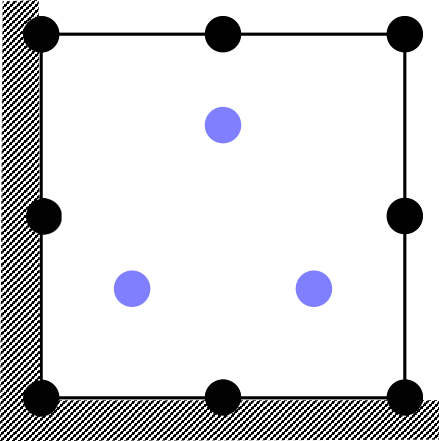
\includegraphics[width=0.3\textwidth]{figures/Q8P3.png} &
            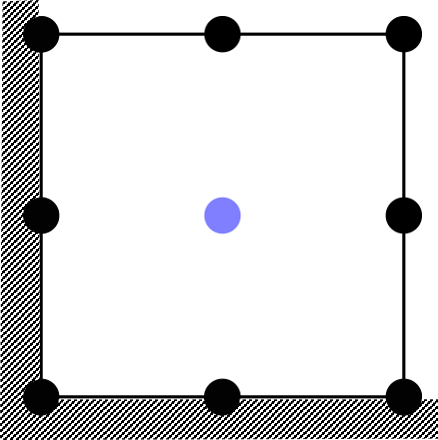
\includegraphics[width=0.3\textwidth]{figures/Q8P1.png} \\
            (a) & (b) \\
            \raisebox{-0.3\height}{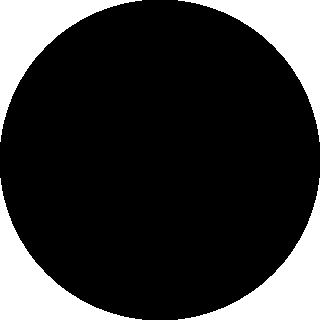
\includegraphics[width=14pt]{figures/legend_u.png}} :位移节点 &
            \raisebox{-0.3\height}{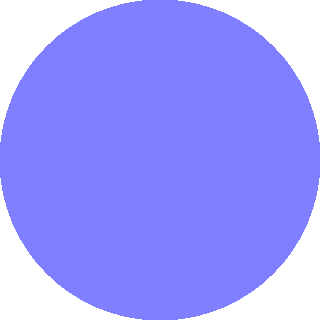
\includegraphics[width=14pt]{figures/legend_p.png}} :压力节点 
        \end{tabular}
        \caption{二维位移压力单元示例}\label{ch_3:fig:elements_eg}
 \end{figure}

表\ref{ch_3:tab:infsup2}为其他经典单元的验证结果,通过对比分析可以看出,本文所提的考虑约束比的LBB稳定性条件,其验证结果与数值验证方法和解析证明方法完全一致。这一结果初步表明,新方法在使用简易的同时,能够验证混合离散方案的LBB稳定性条件。
\begin{table}[!h]
    \centering
    \renewcommand\arraystretch{1.2}
    \caption{LBB稳定性条件验证} \label{ch_3:tab:infsup2}
    \begin{tabular}{ccccc}
        \hline
        \multirow{2}{*}{离散方案}&体积&\multicolumn{2}{c}{LBB稳定性条件}&考虑约束比的\\
        & 约束比&数值验证&解析证明&LBB稳定性条件\\
        \hline
        \begin{tabular}{c}
            \begin{minipage}{0.13\columnwidth}
                \centering
                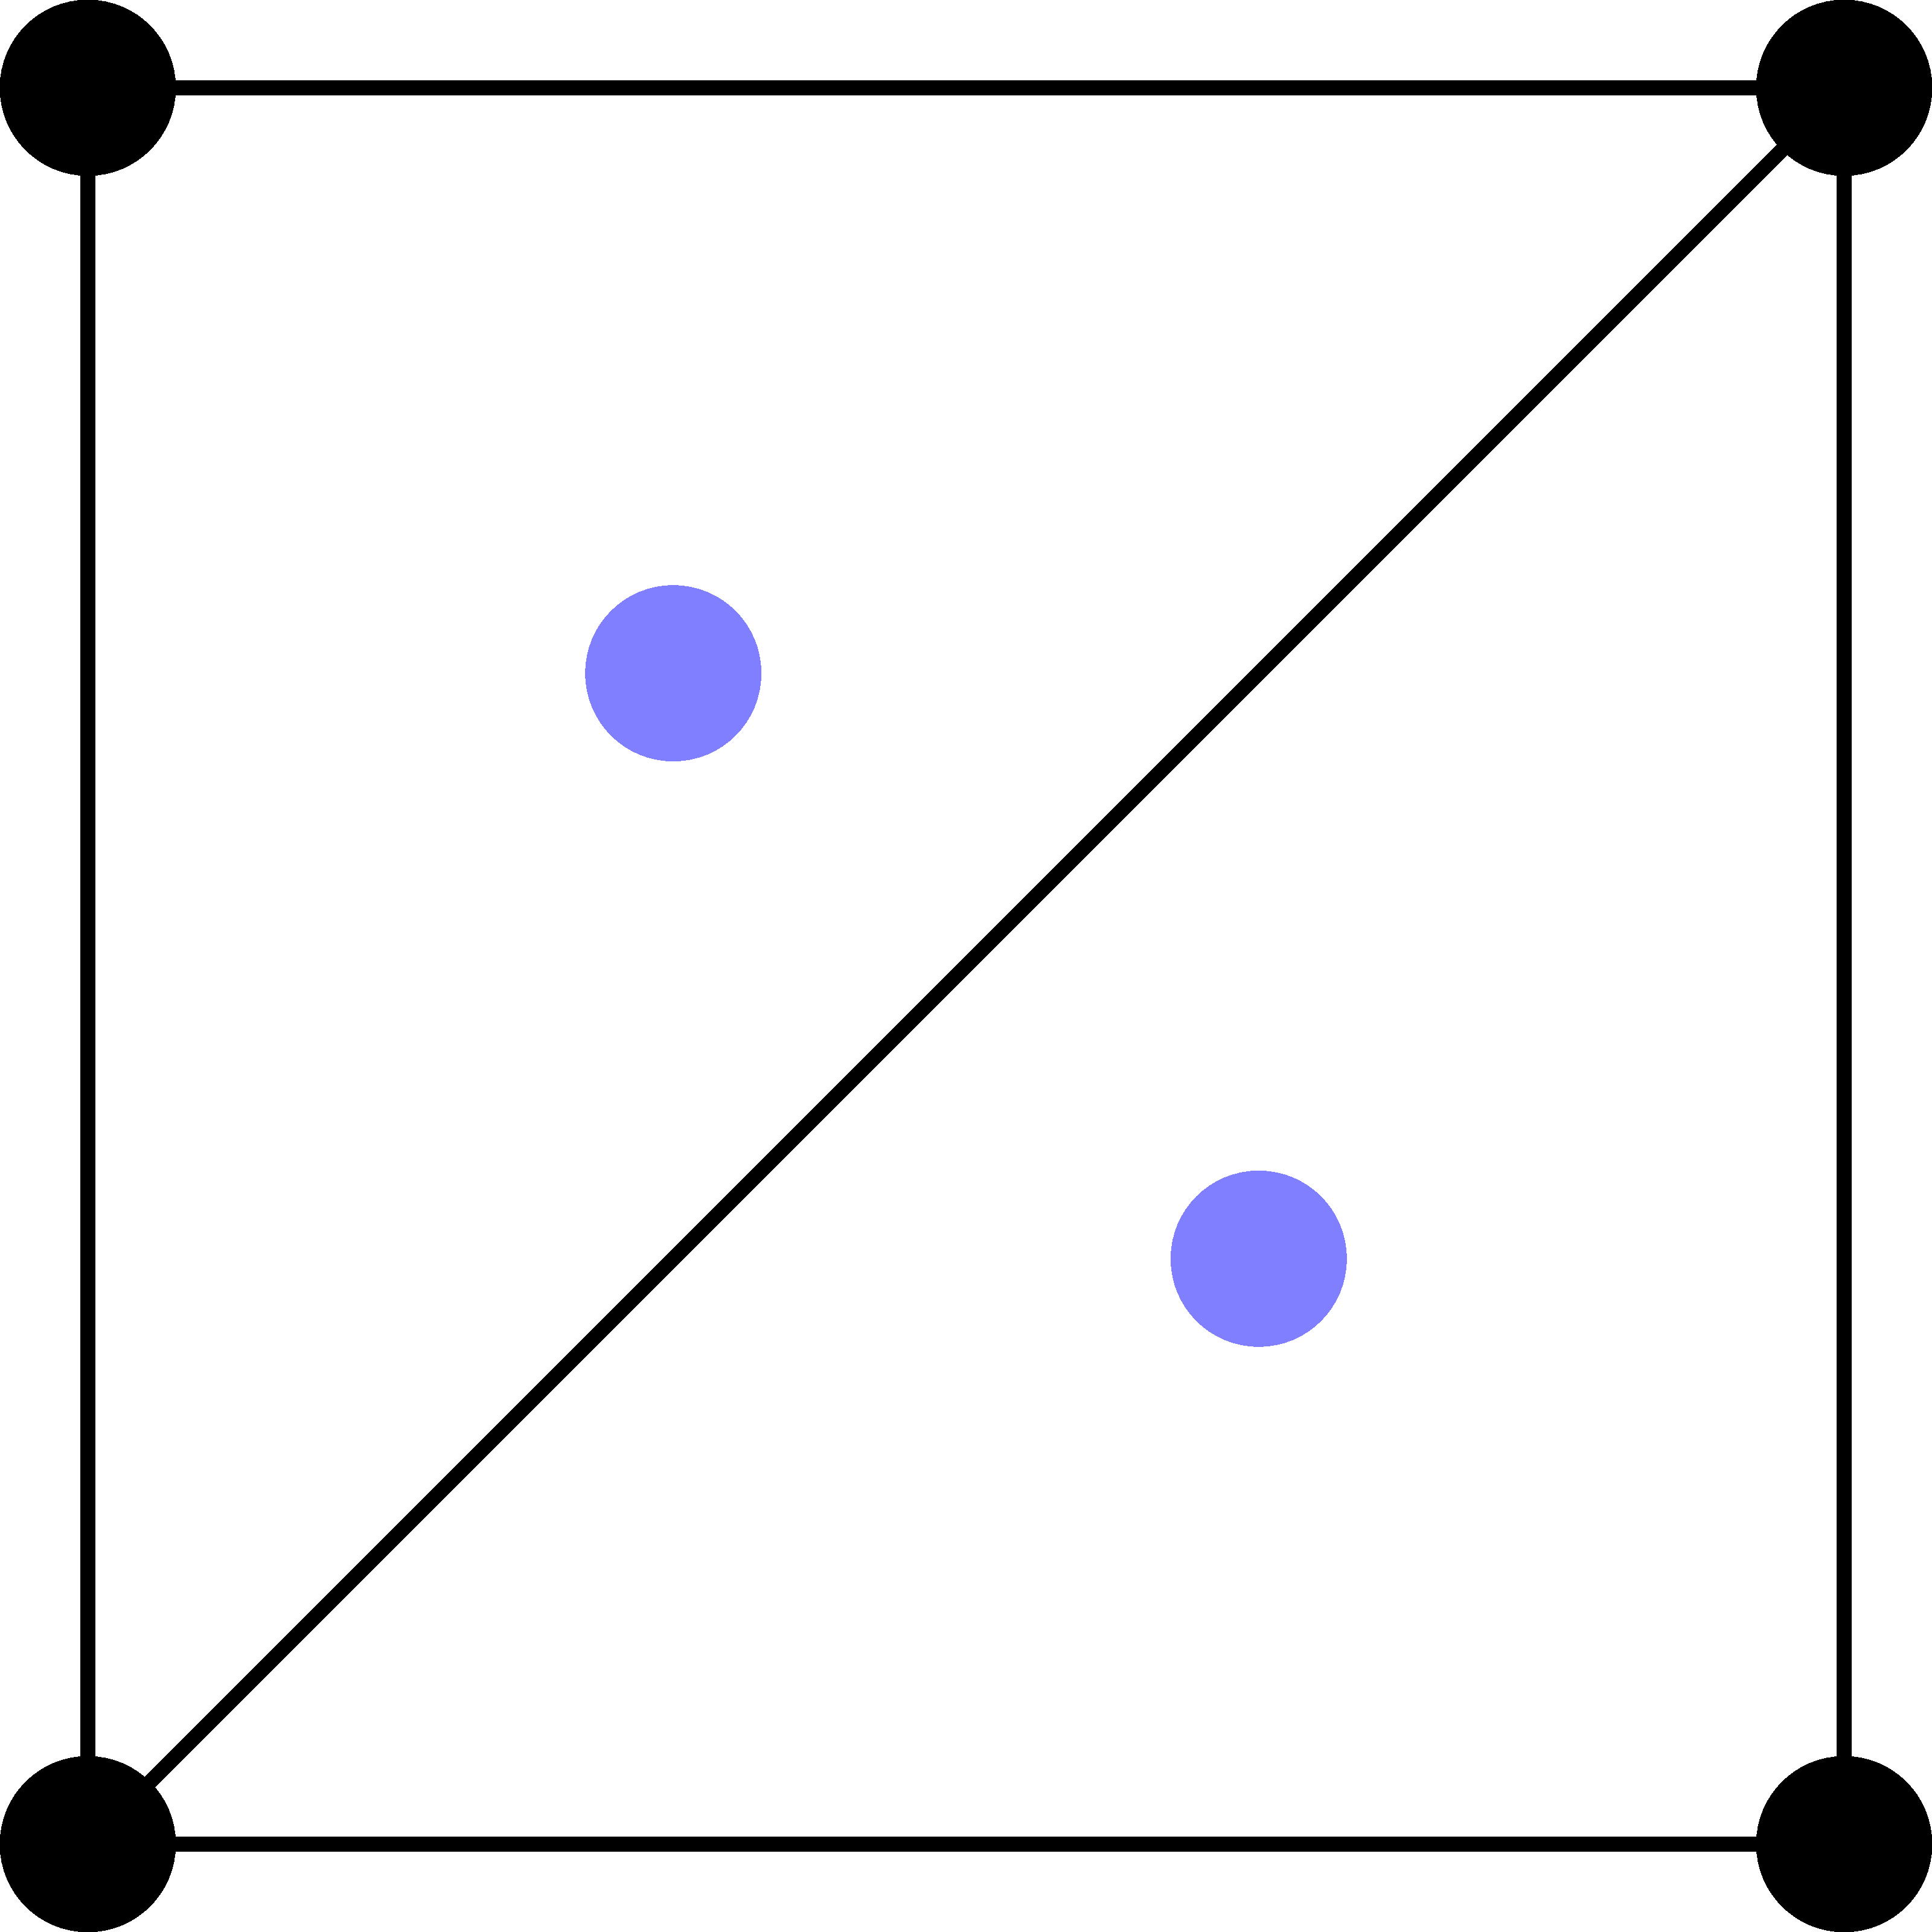
\includegraphics[width=0.9\textwidth]{figures/mix_T3P1.png}
            \end{minipage}\\T3P1
        \end{tabular}
        &1&$\times$ & $\times$&$\times$\\
        \begin{tabular}{c}
            \begin{minipage}{0.13\columnwidth}
                \centering
                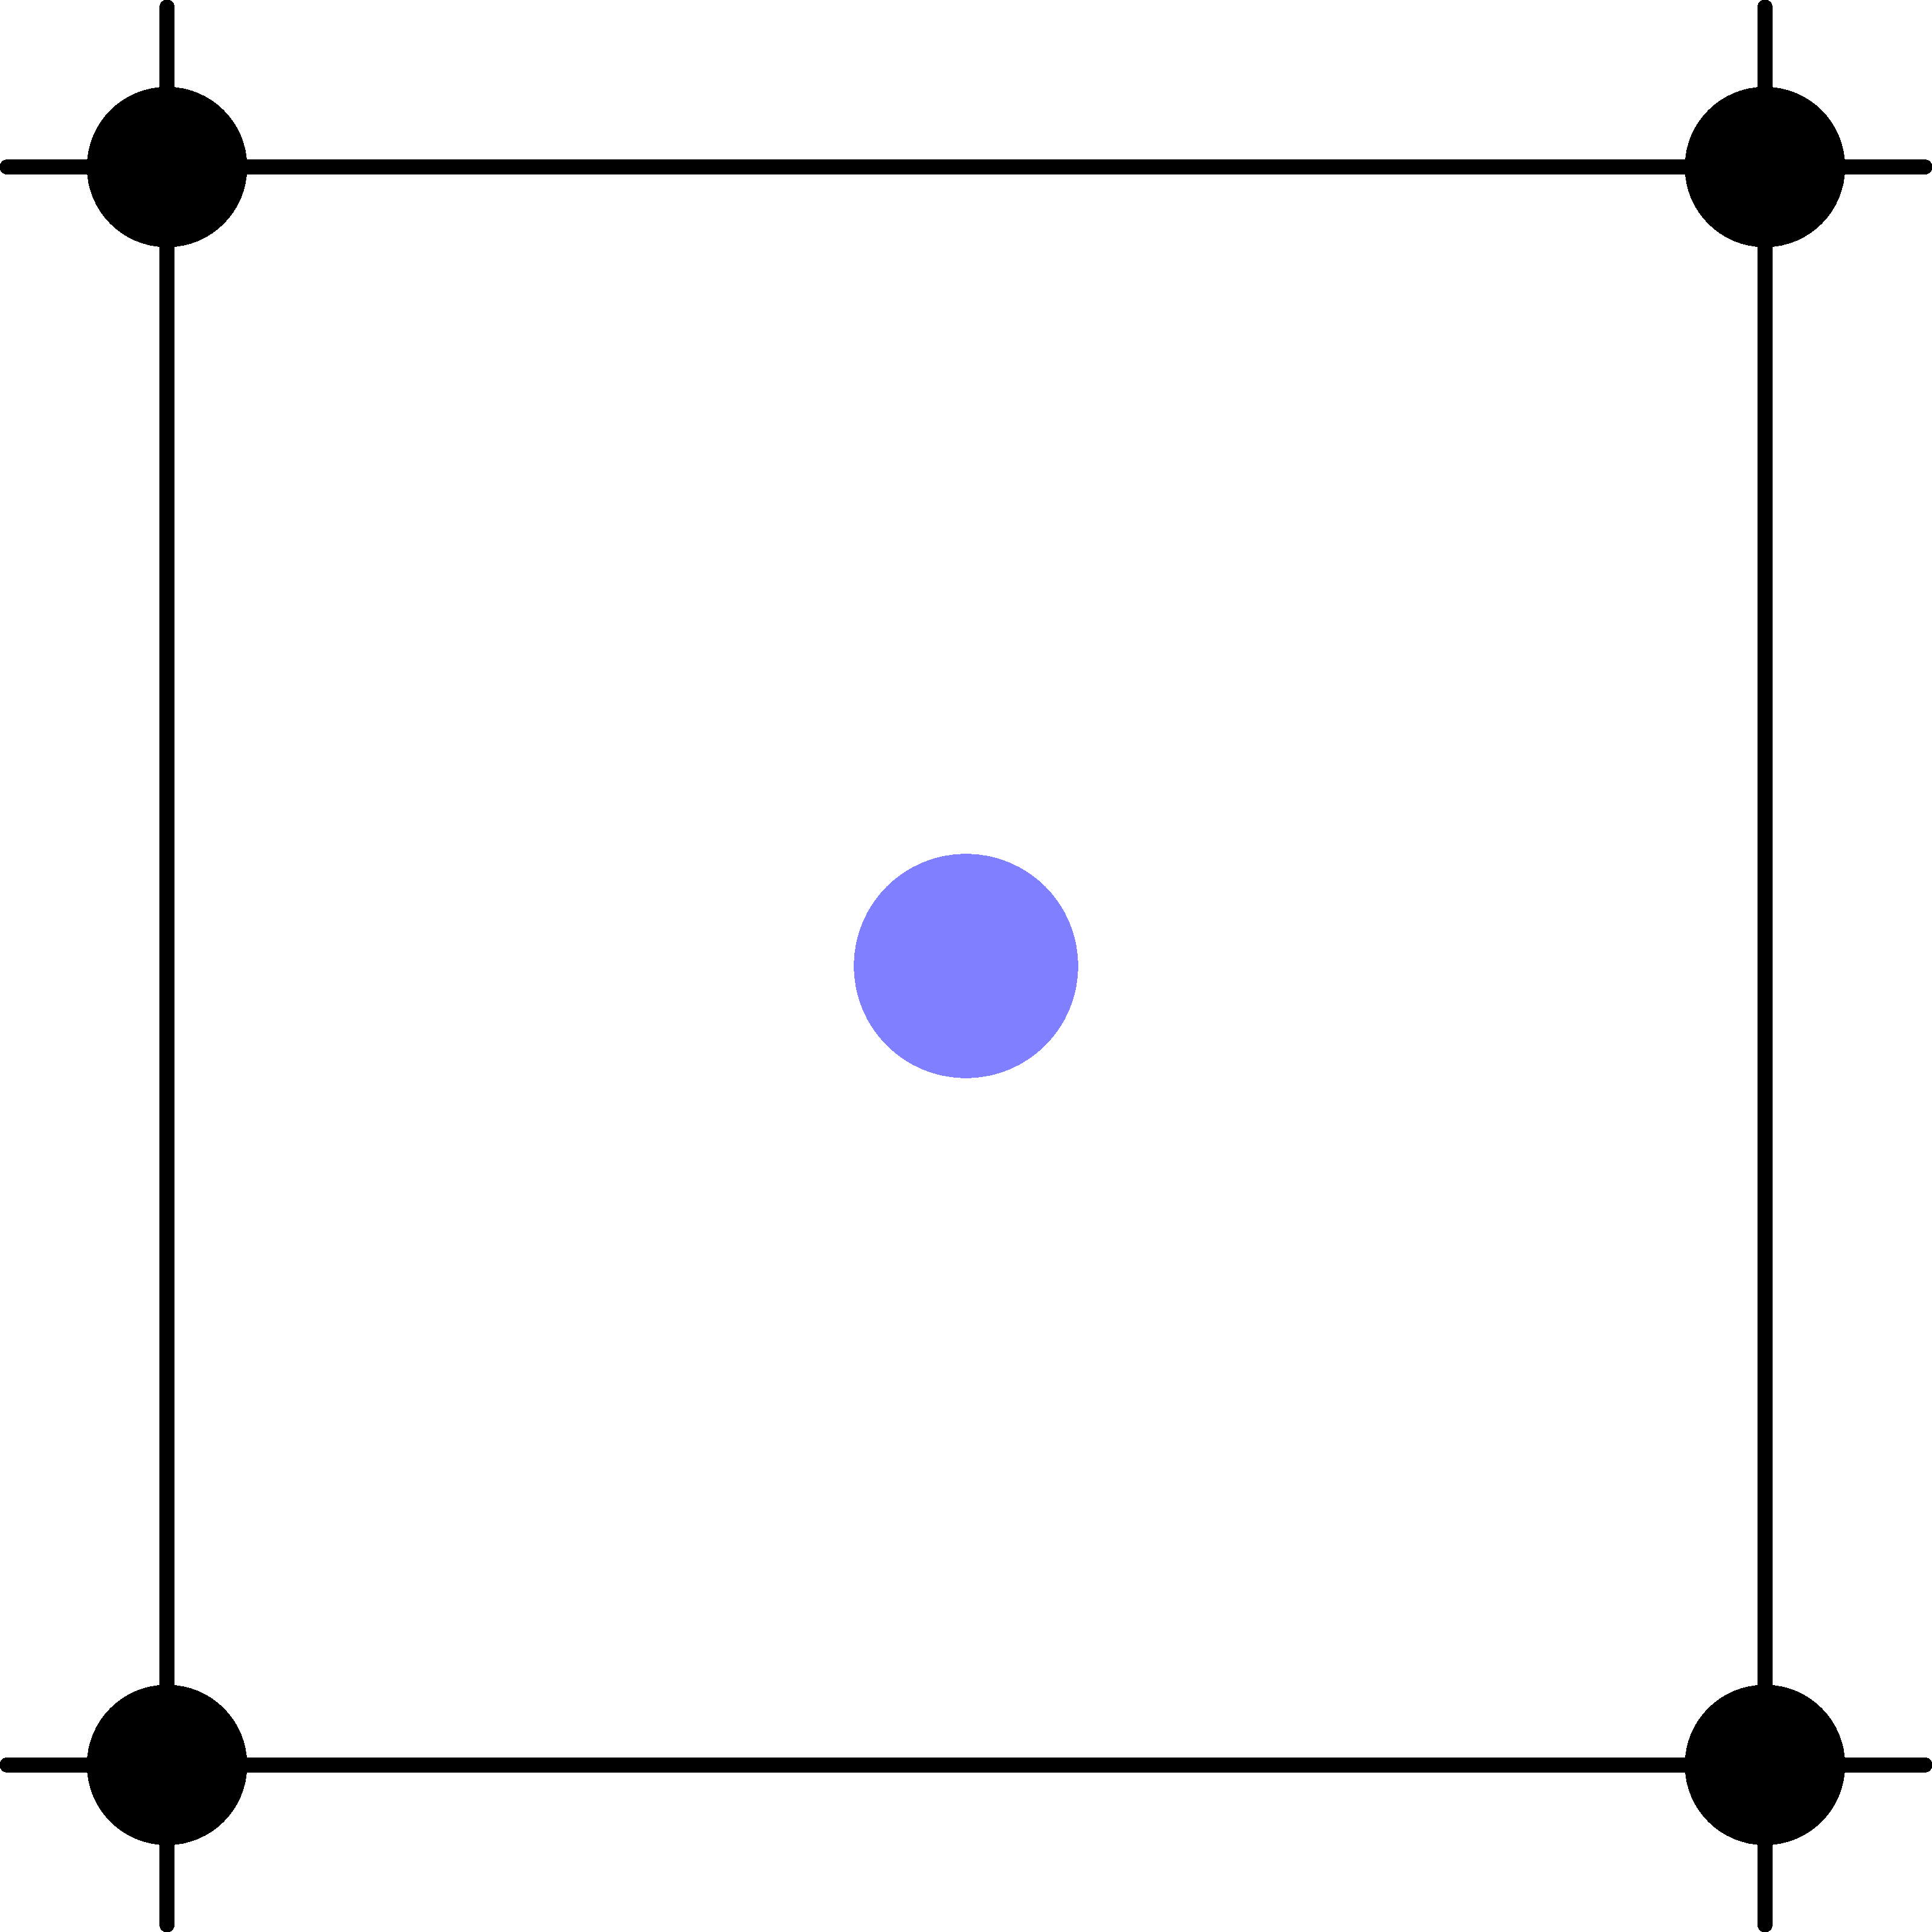
\includegraphics[width=0.9\textwidth]{figures/mix_Q4P1.png}
            \end{minipage}\\Q4P1
        \end{tabular}
        &2&$\times$ & $\times$&$\times$\\
        \begin{tabular}{c}
            \begin{minipage}{0.13\columnwidth}
                \centering
                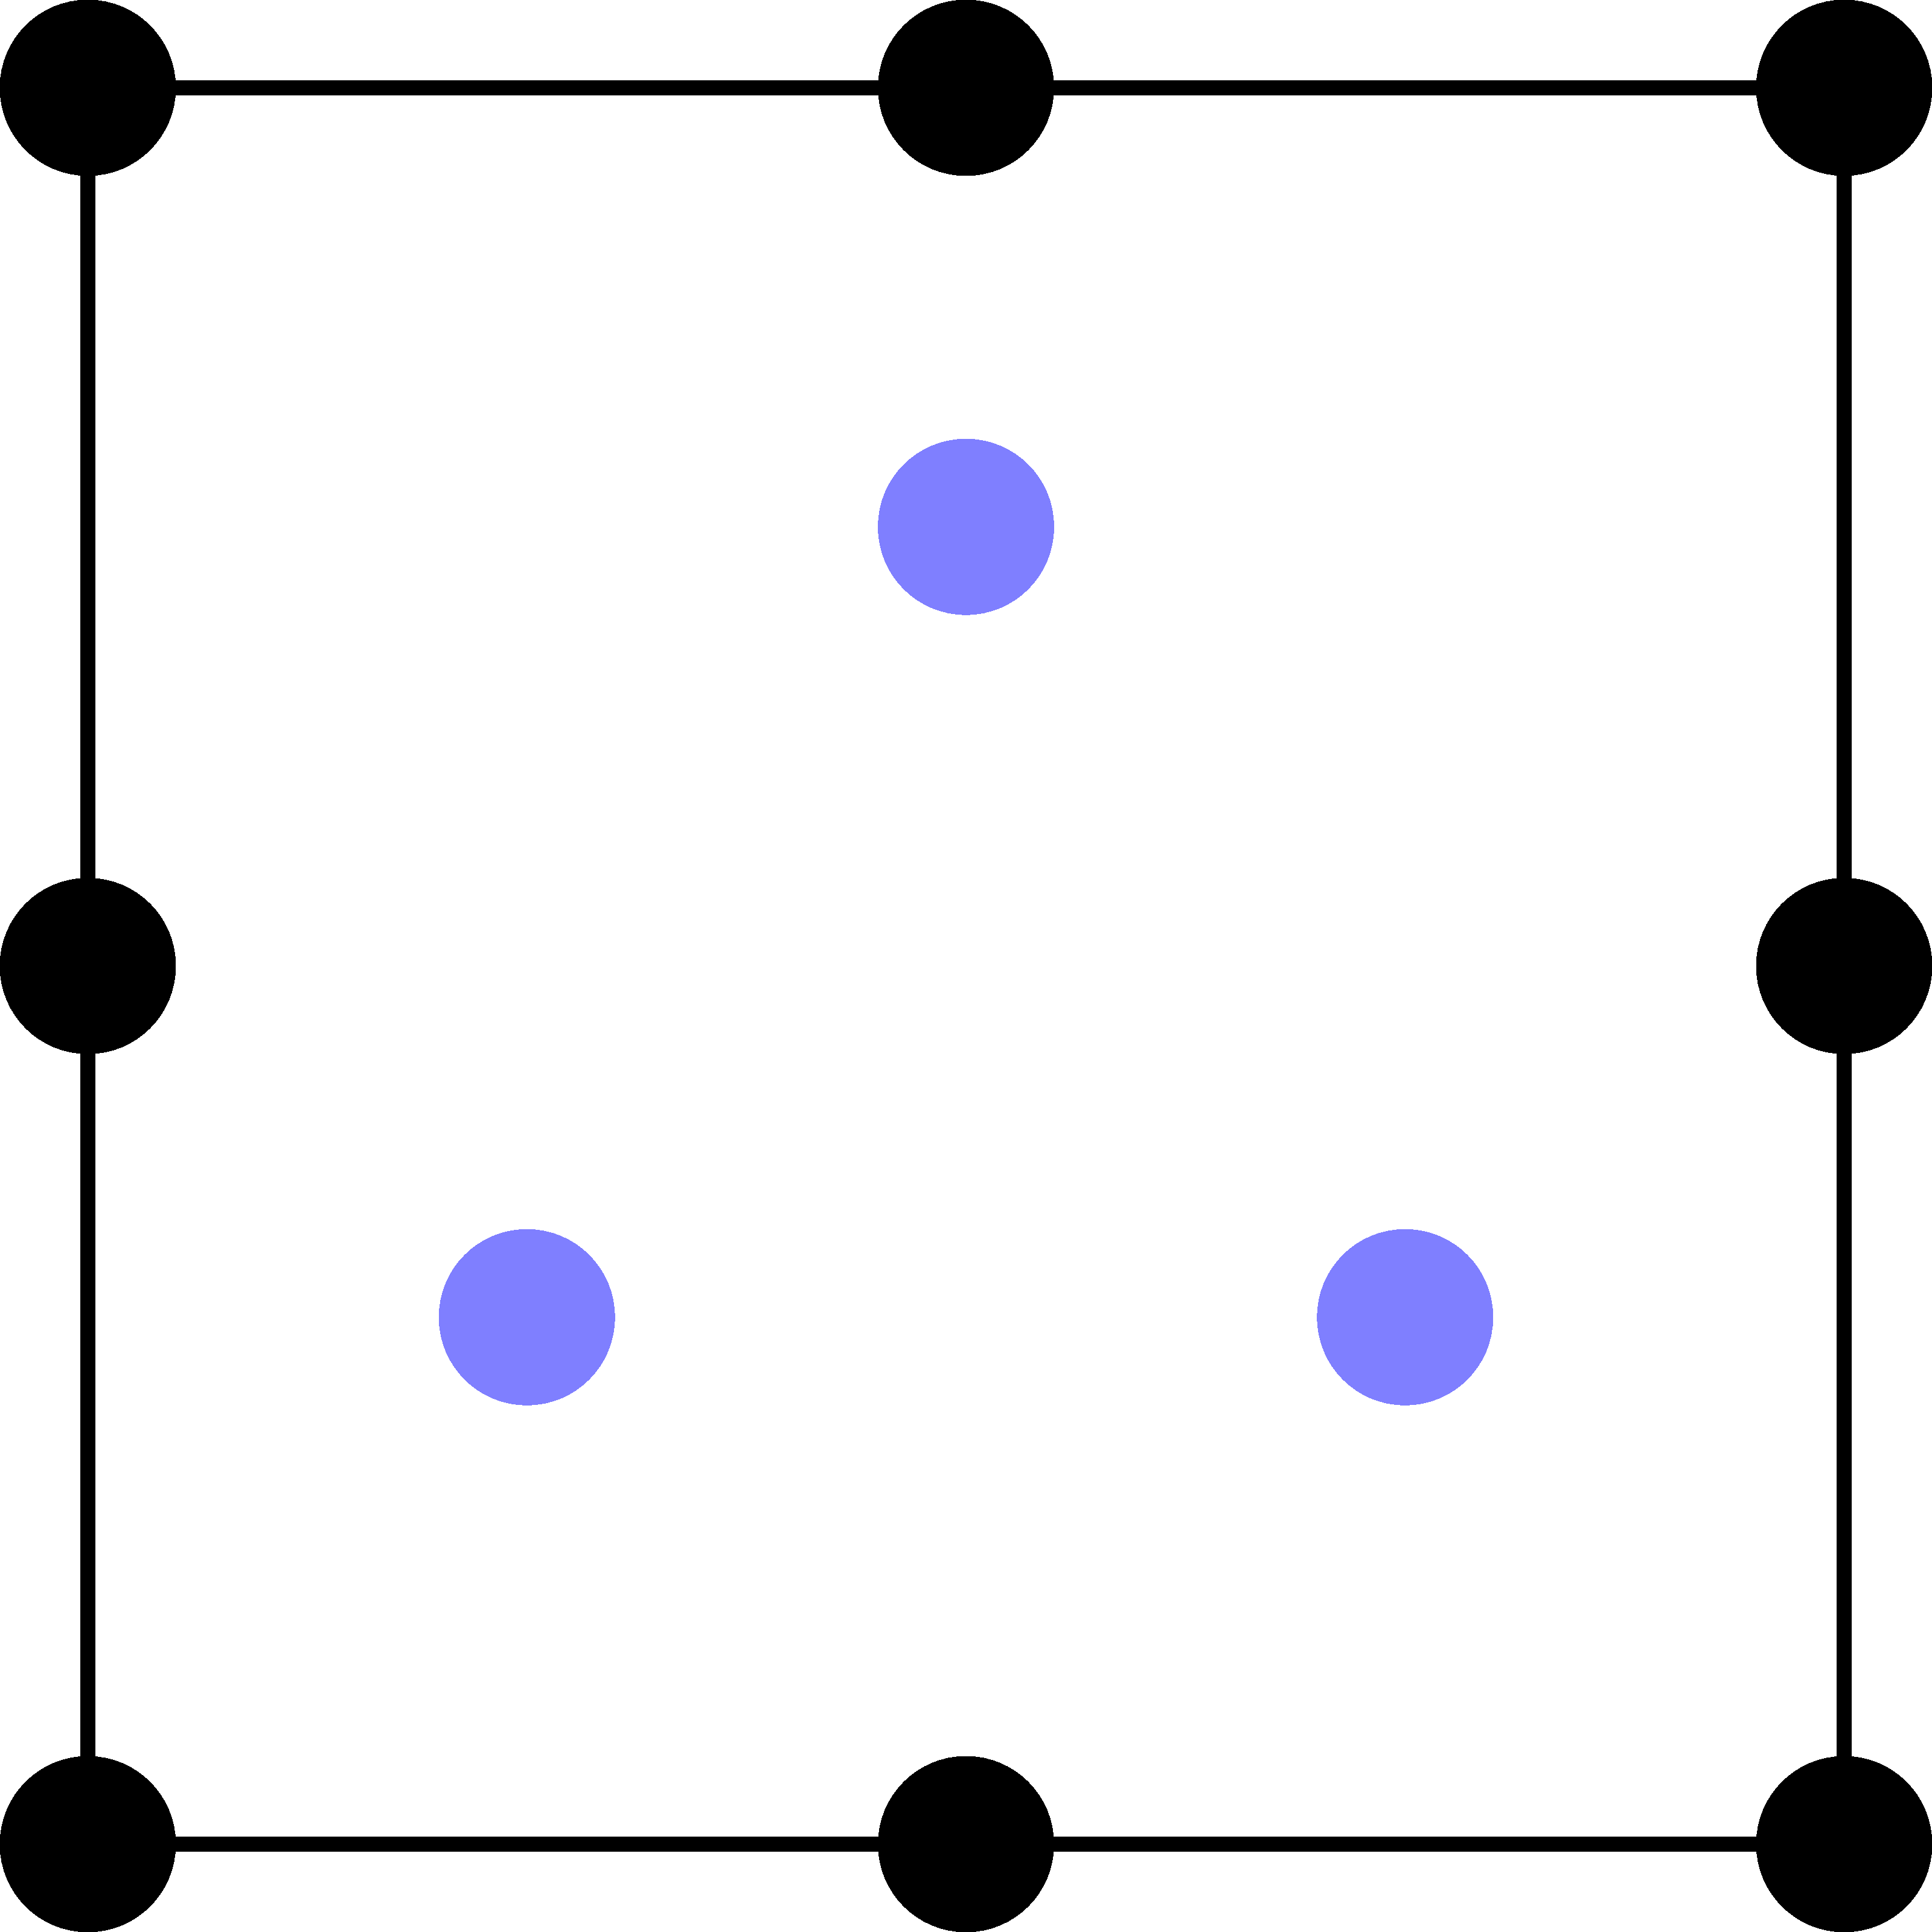
\includegraphics[width=0.9\textwidth]{figures/mix_Q8P3.png}
            \end{minipage}\\Q8P3
        \end{tabular}
        &2&$\times$ & $\times$&$\times$\\
        \begin{tabular}{c}
            \begin{minipage}{0.13\columnwidth}
                \centering
                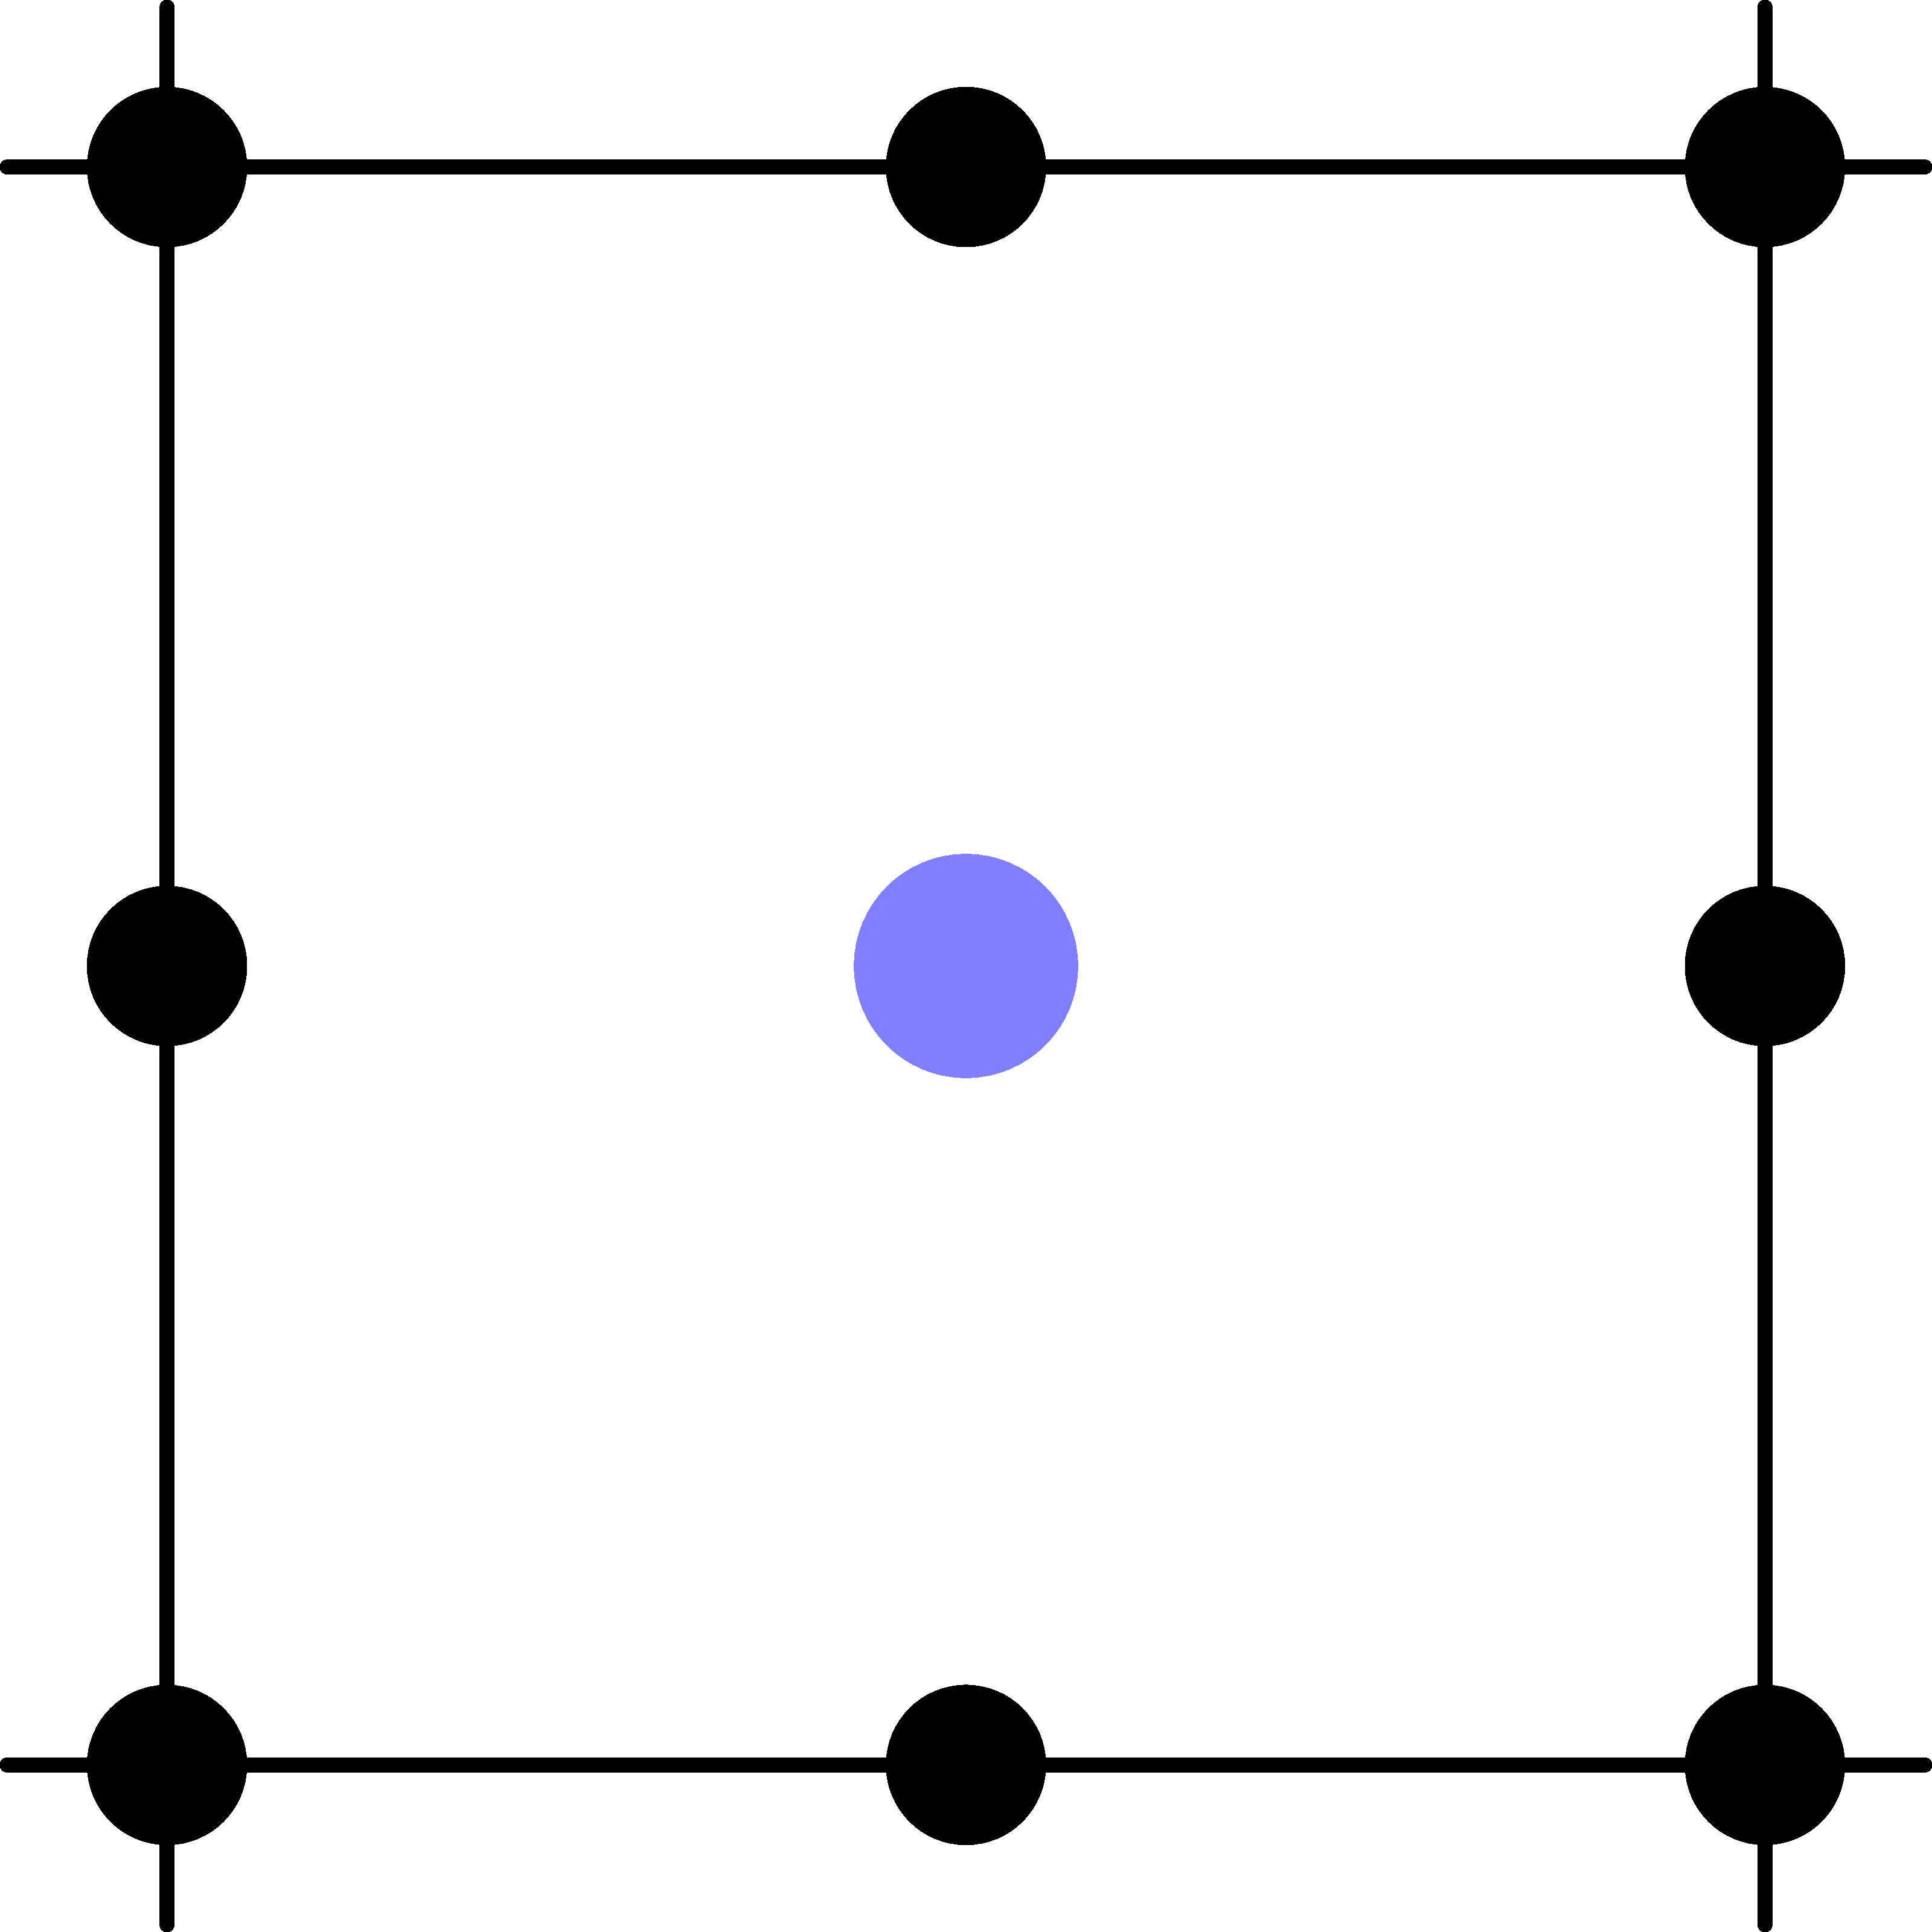
\includegraphics[width=0.9\textwidth]{figures/mix_Q8P1.png}
            \end{minipage}\\Q8P1
        \end{tabular}
        &6&\checkmark & \checkmark & \checkmark\\
        \begin{tabular}{c}
            \begin{minipage}{0.13\columnwidth}
                \centering
                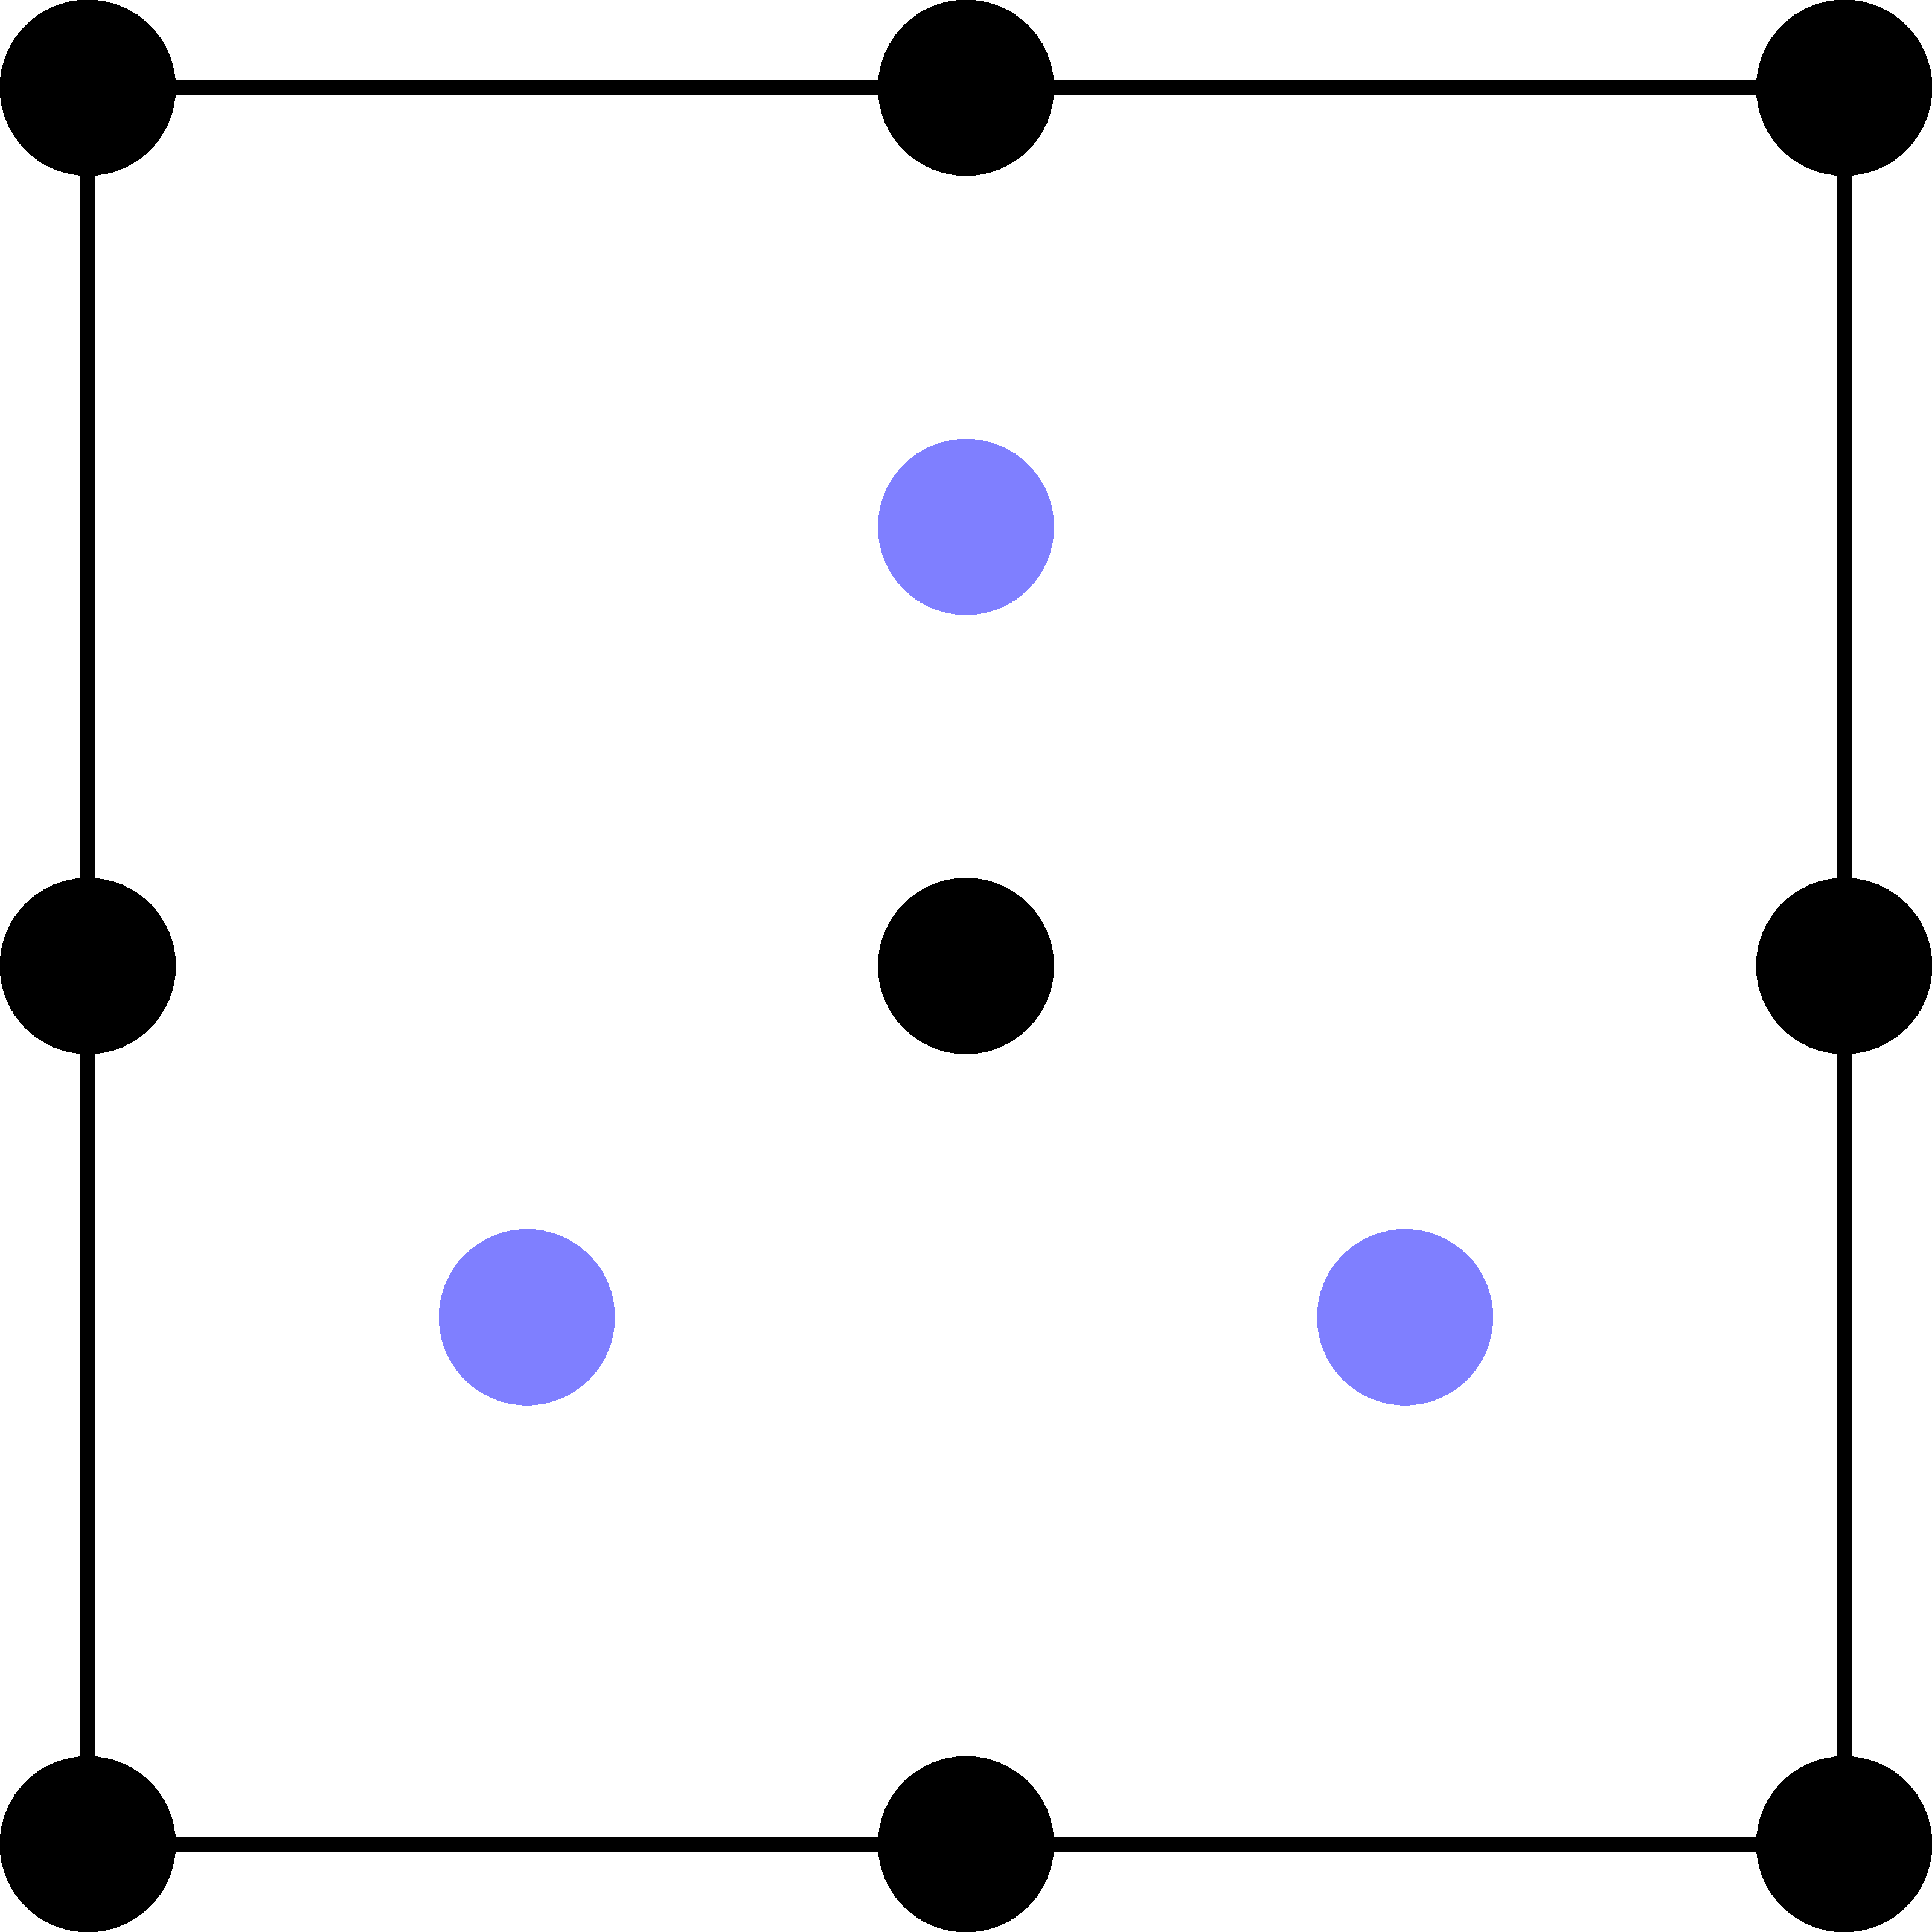
\includegraphics[width=0.9\textwidth]{figures/mix_Q9P3.png}
            \end{minipage}\\Q9P3
        \end{tabular}
        &$\frac{8}{3}$&\checkmark & \checkmark & \checkmark\\
        \begin{tabular}{c}
            \begin{minipage}{0.13\columnwidth}
                \centering
                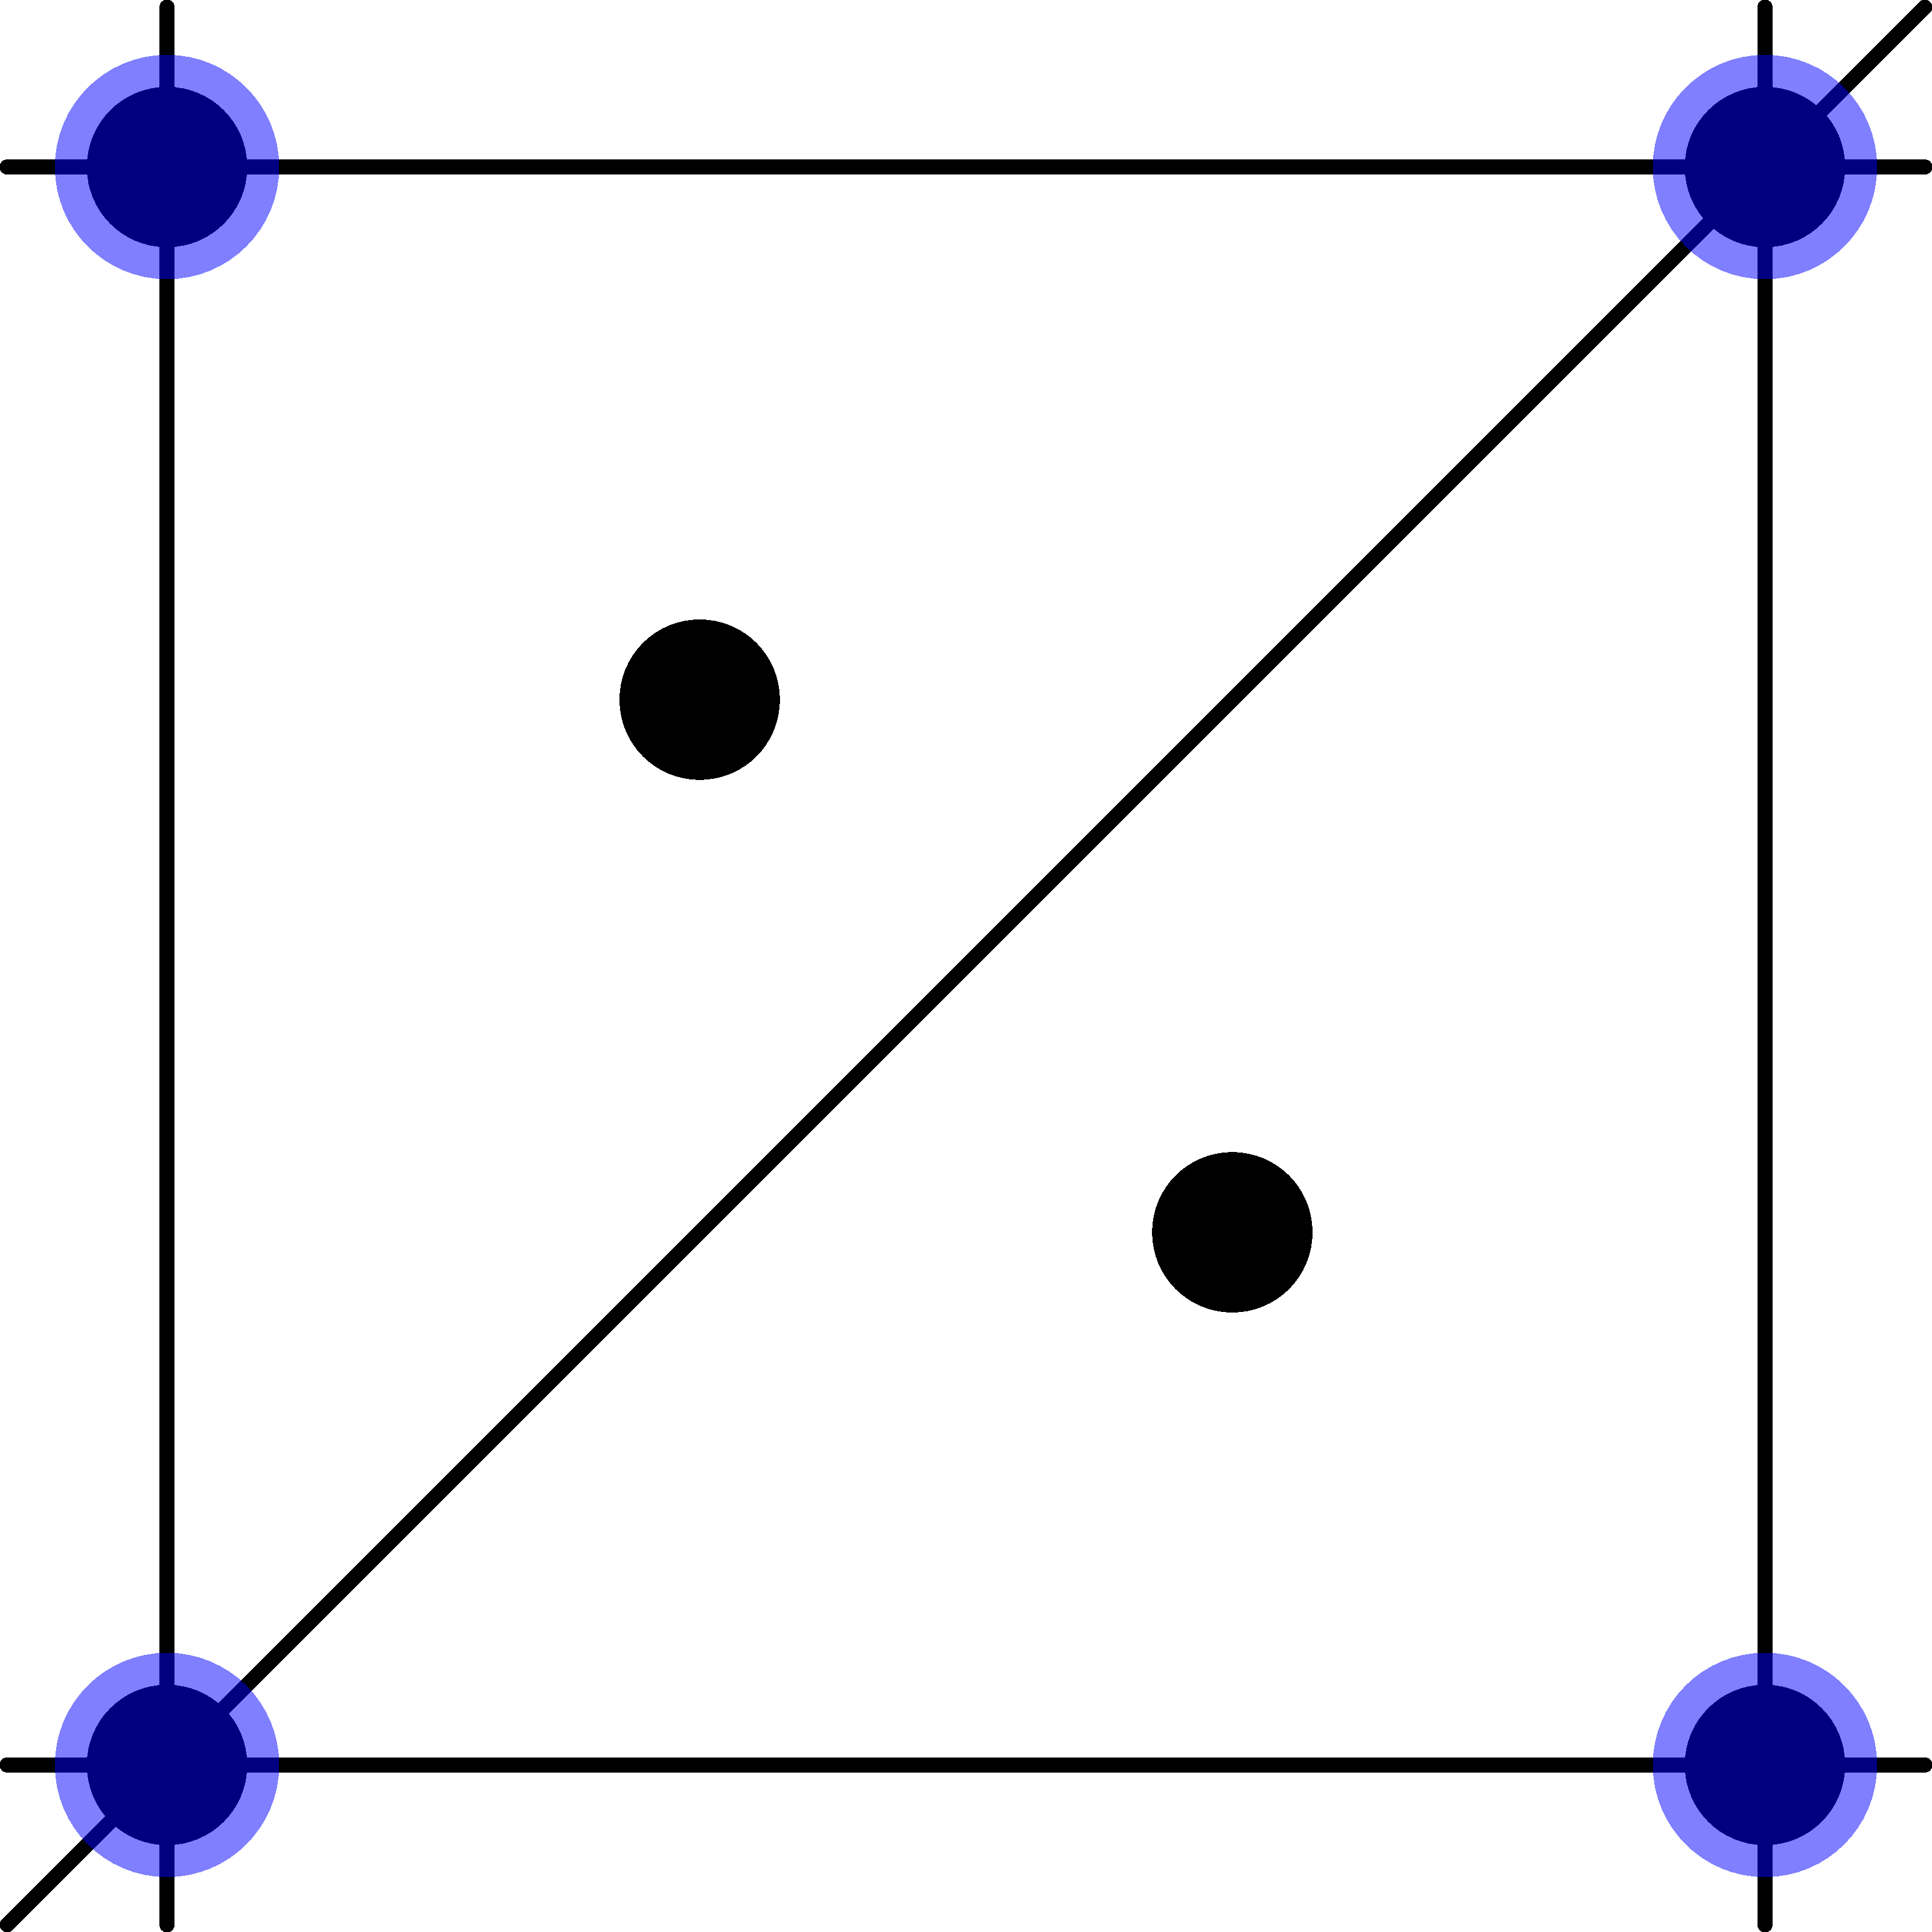
\includegraphics[width=0.9\textwidth]{figures/mini.png}
            \end{minipage}\\MINI element \cite{arnold1984,auricchio2005}
        \end{tabular}
        &$\frac{8}{3}$&\checkmark & \checkmark& \checkmark\\
        \begin{tabular}{c}
            \begin{minipage}{0.13\columnwidth}
                \centering
                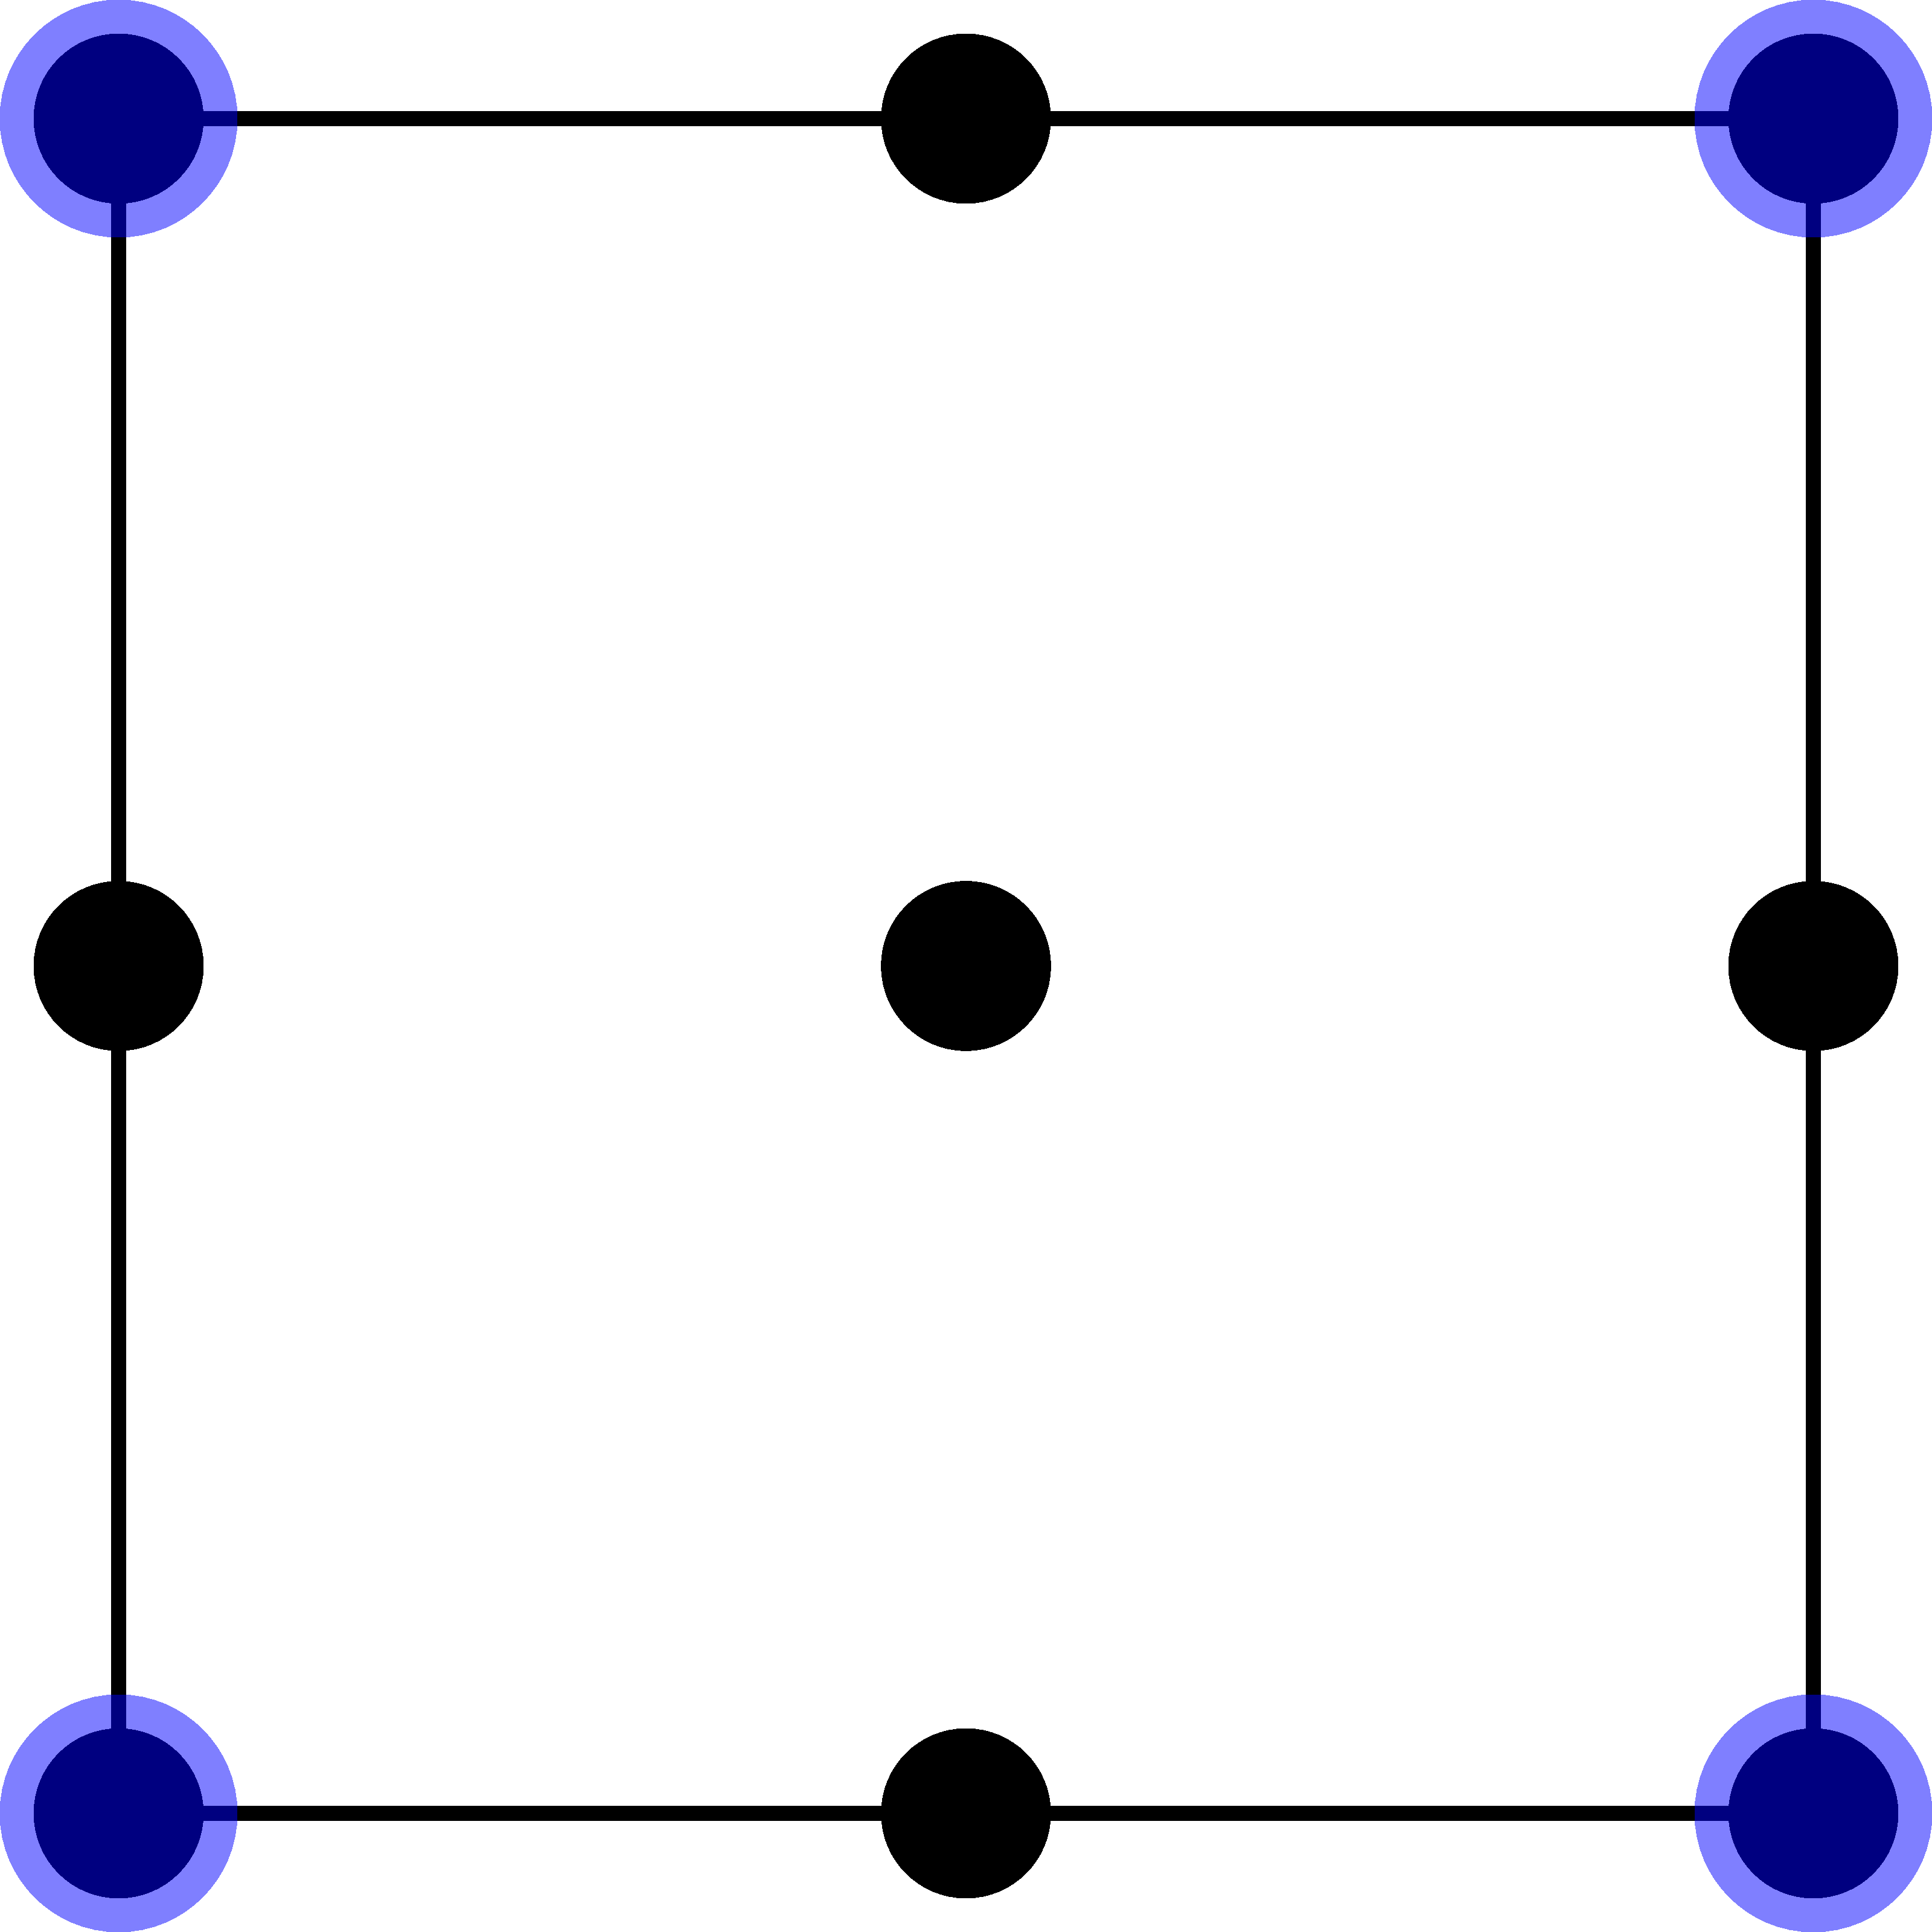
\includegraphics[width=0.9\textwidth]{figures/TaylorHood.png}
            \end{minipage}\\Taylor--Hood element \cite{hood1974}
        \end{tabular}
        &$\frac{8}{3}$&\checkmark & \checkmark& \checkmark\\
        \begin{tabular}{c}
            \begin{minipage}{0.13\columnwidth}
                \centering
                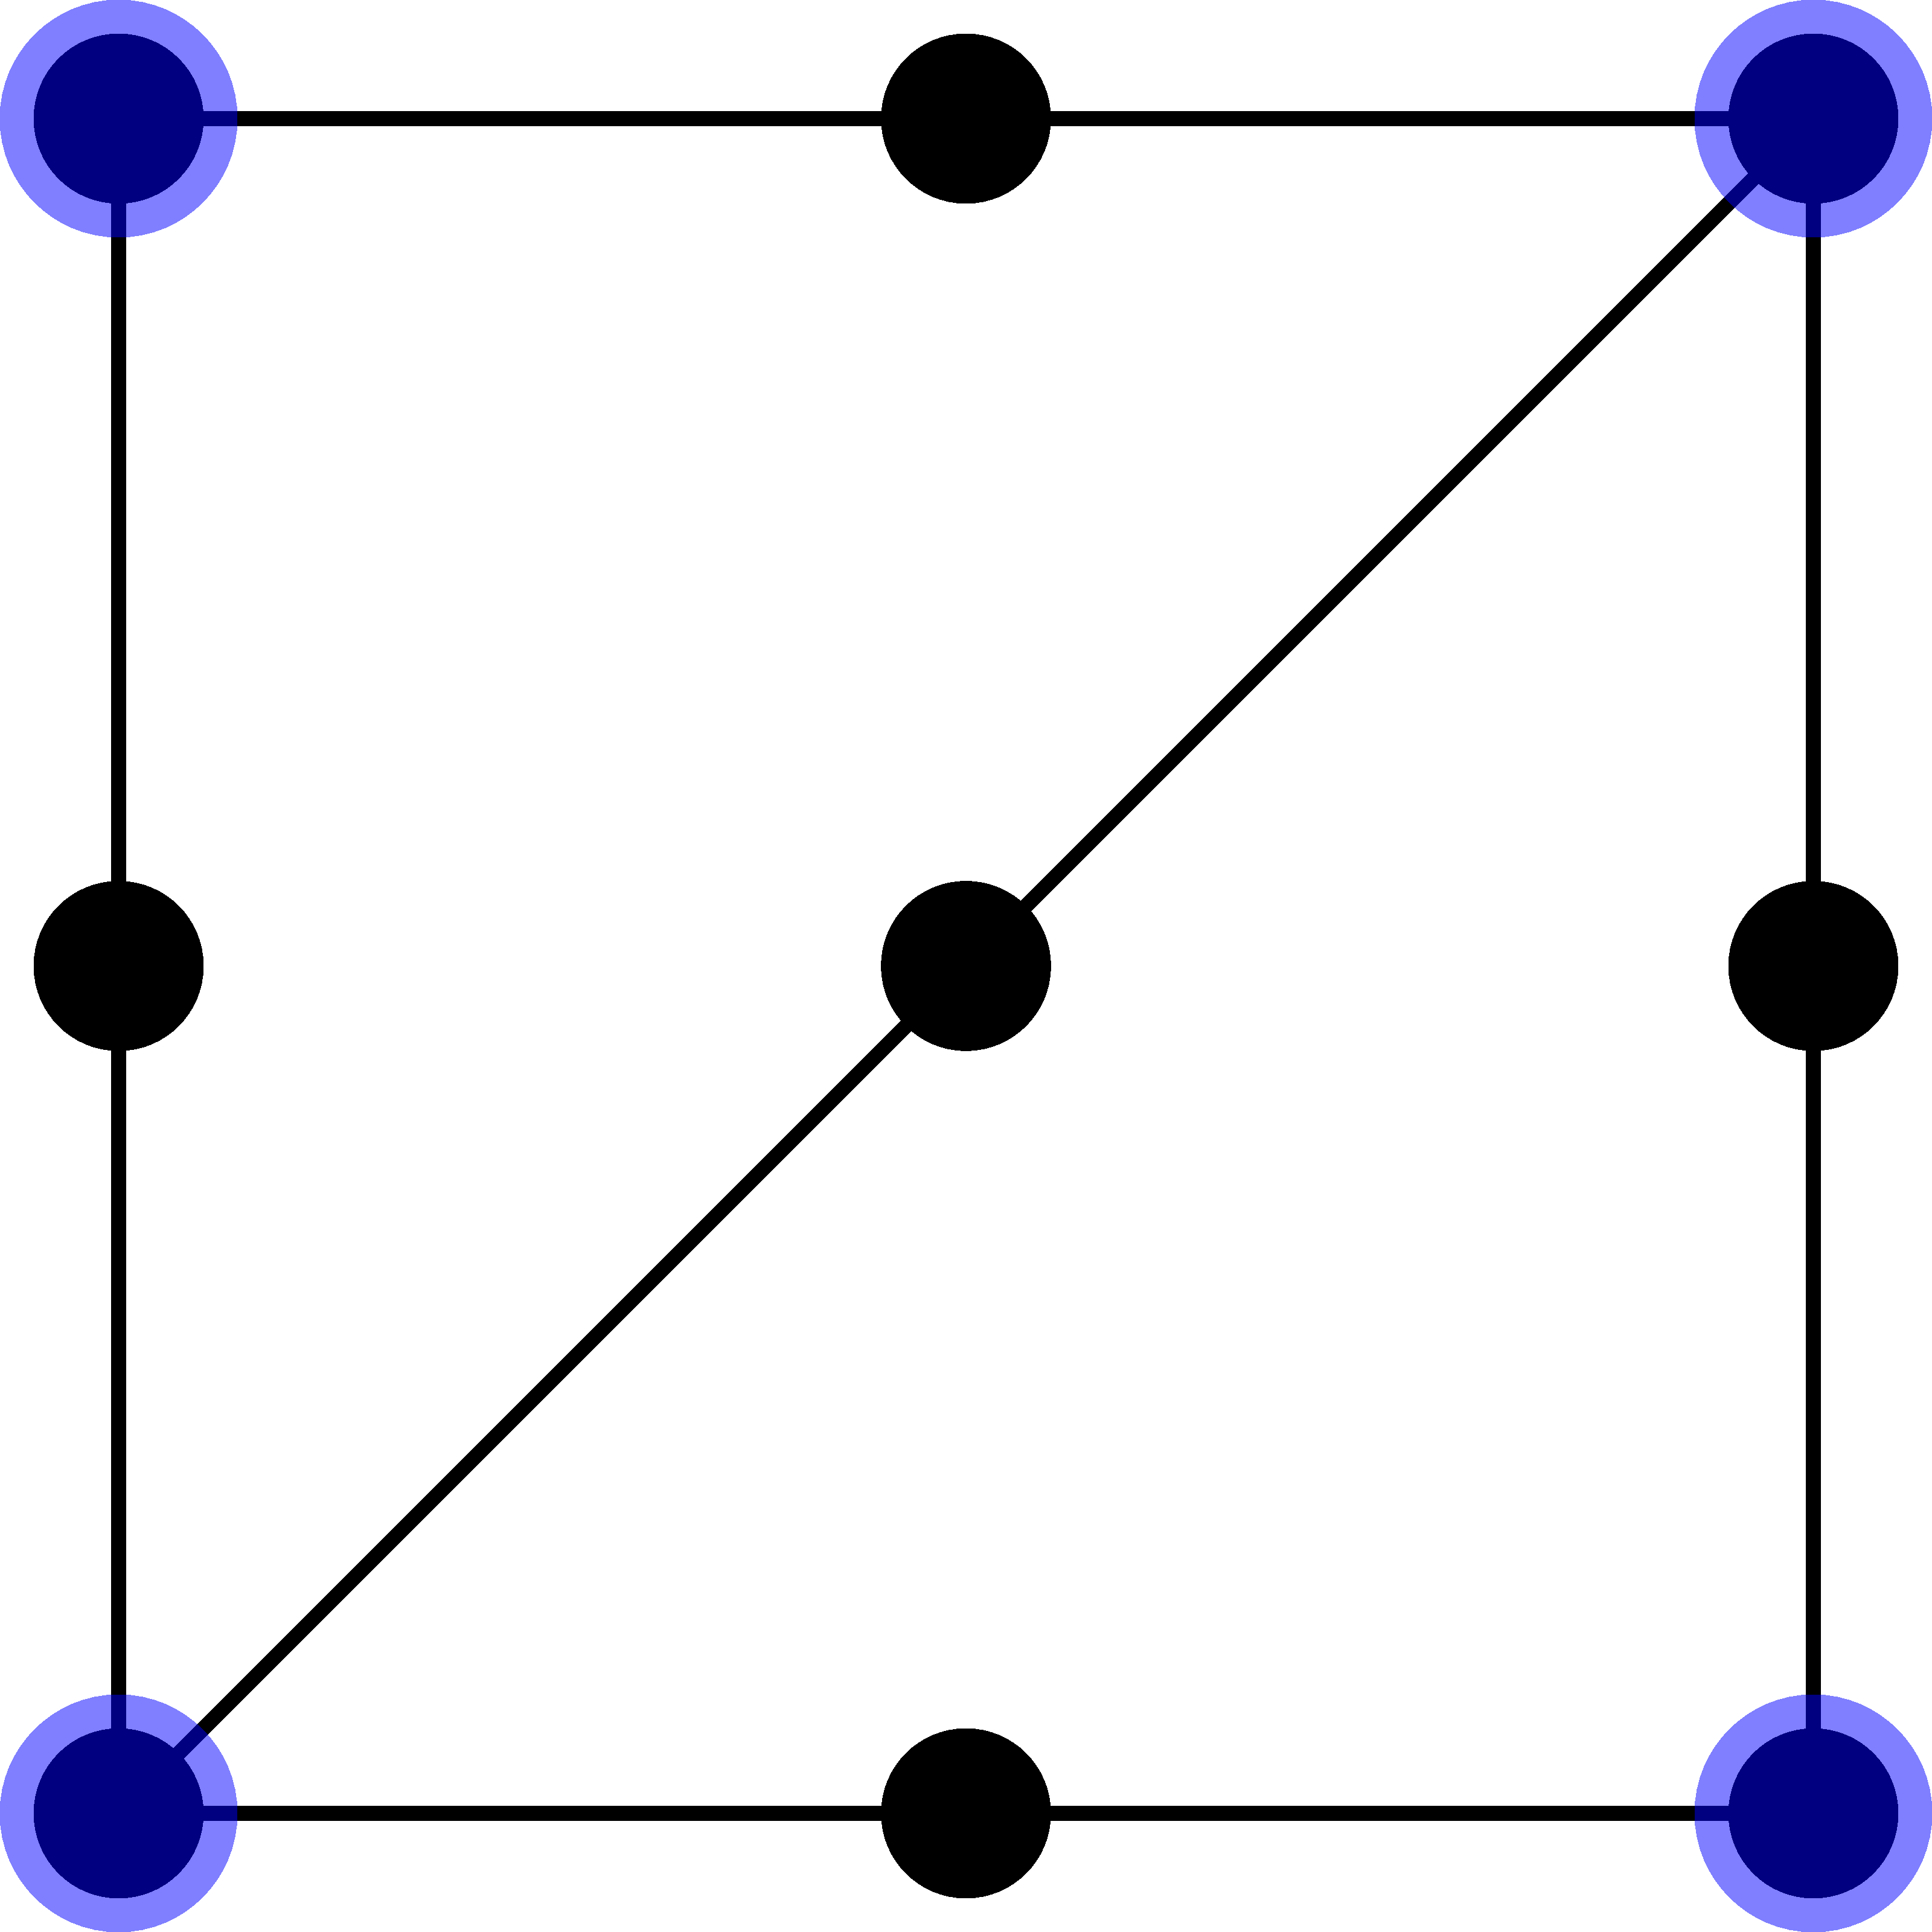
\includegraphics[width=0.9\textwidth]{figures/mix_T6C3.png}
            \end{minipage}\\T6C3
        \end{tabular}
        &8&\checkmark & & \checkmark\\
        \begin{tabular}{c}
            \begin{minipage}{0.13\columnwidth}
                \centering
                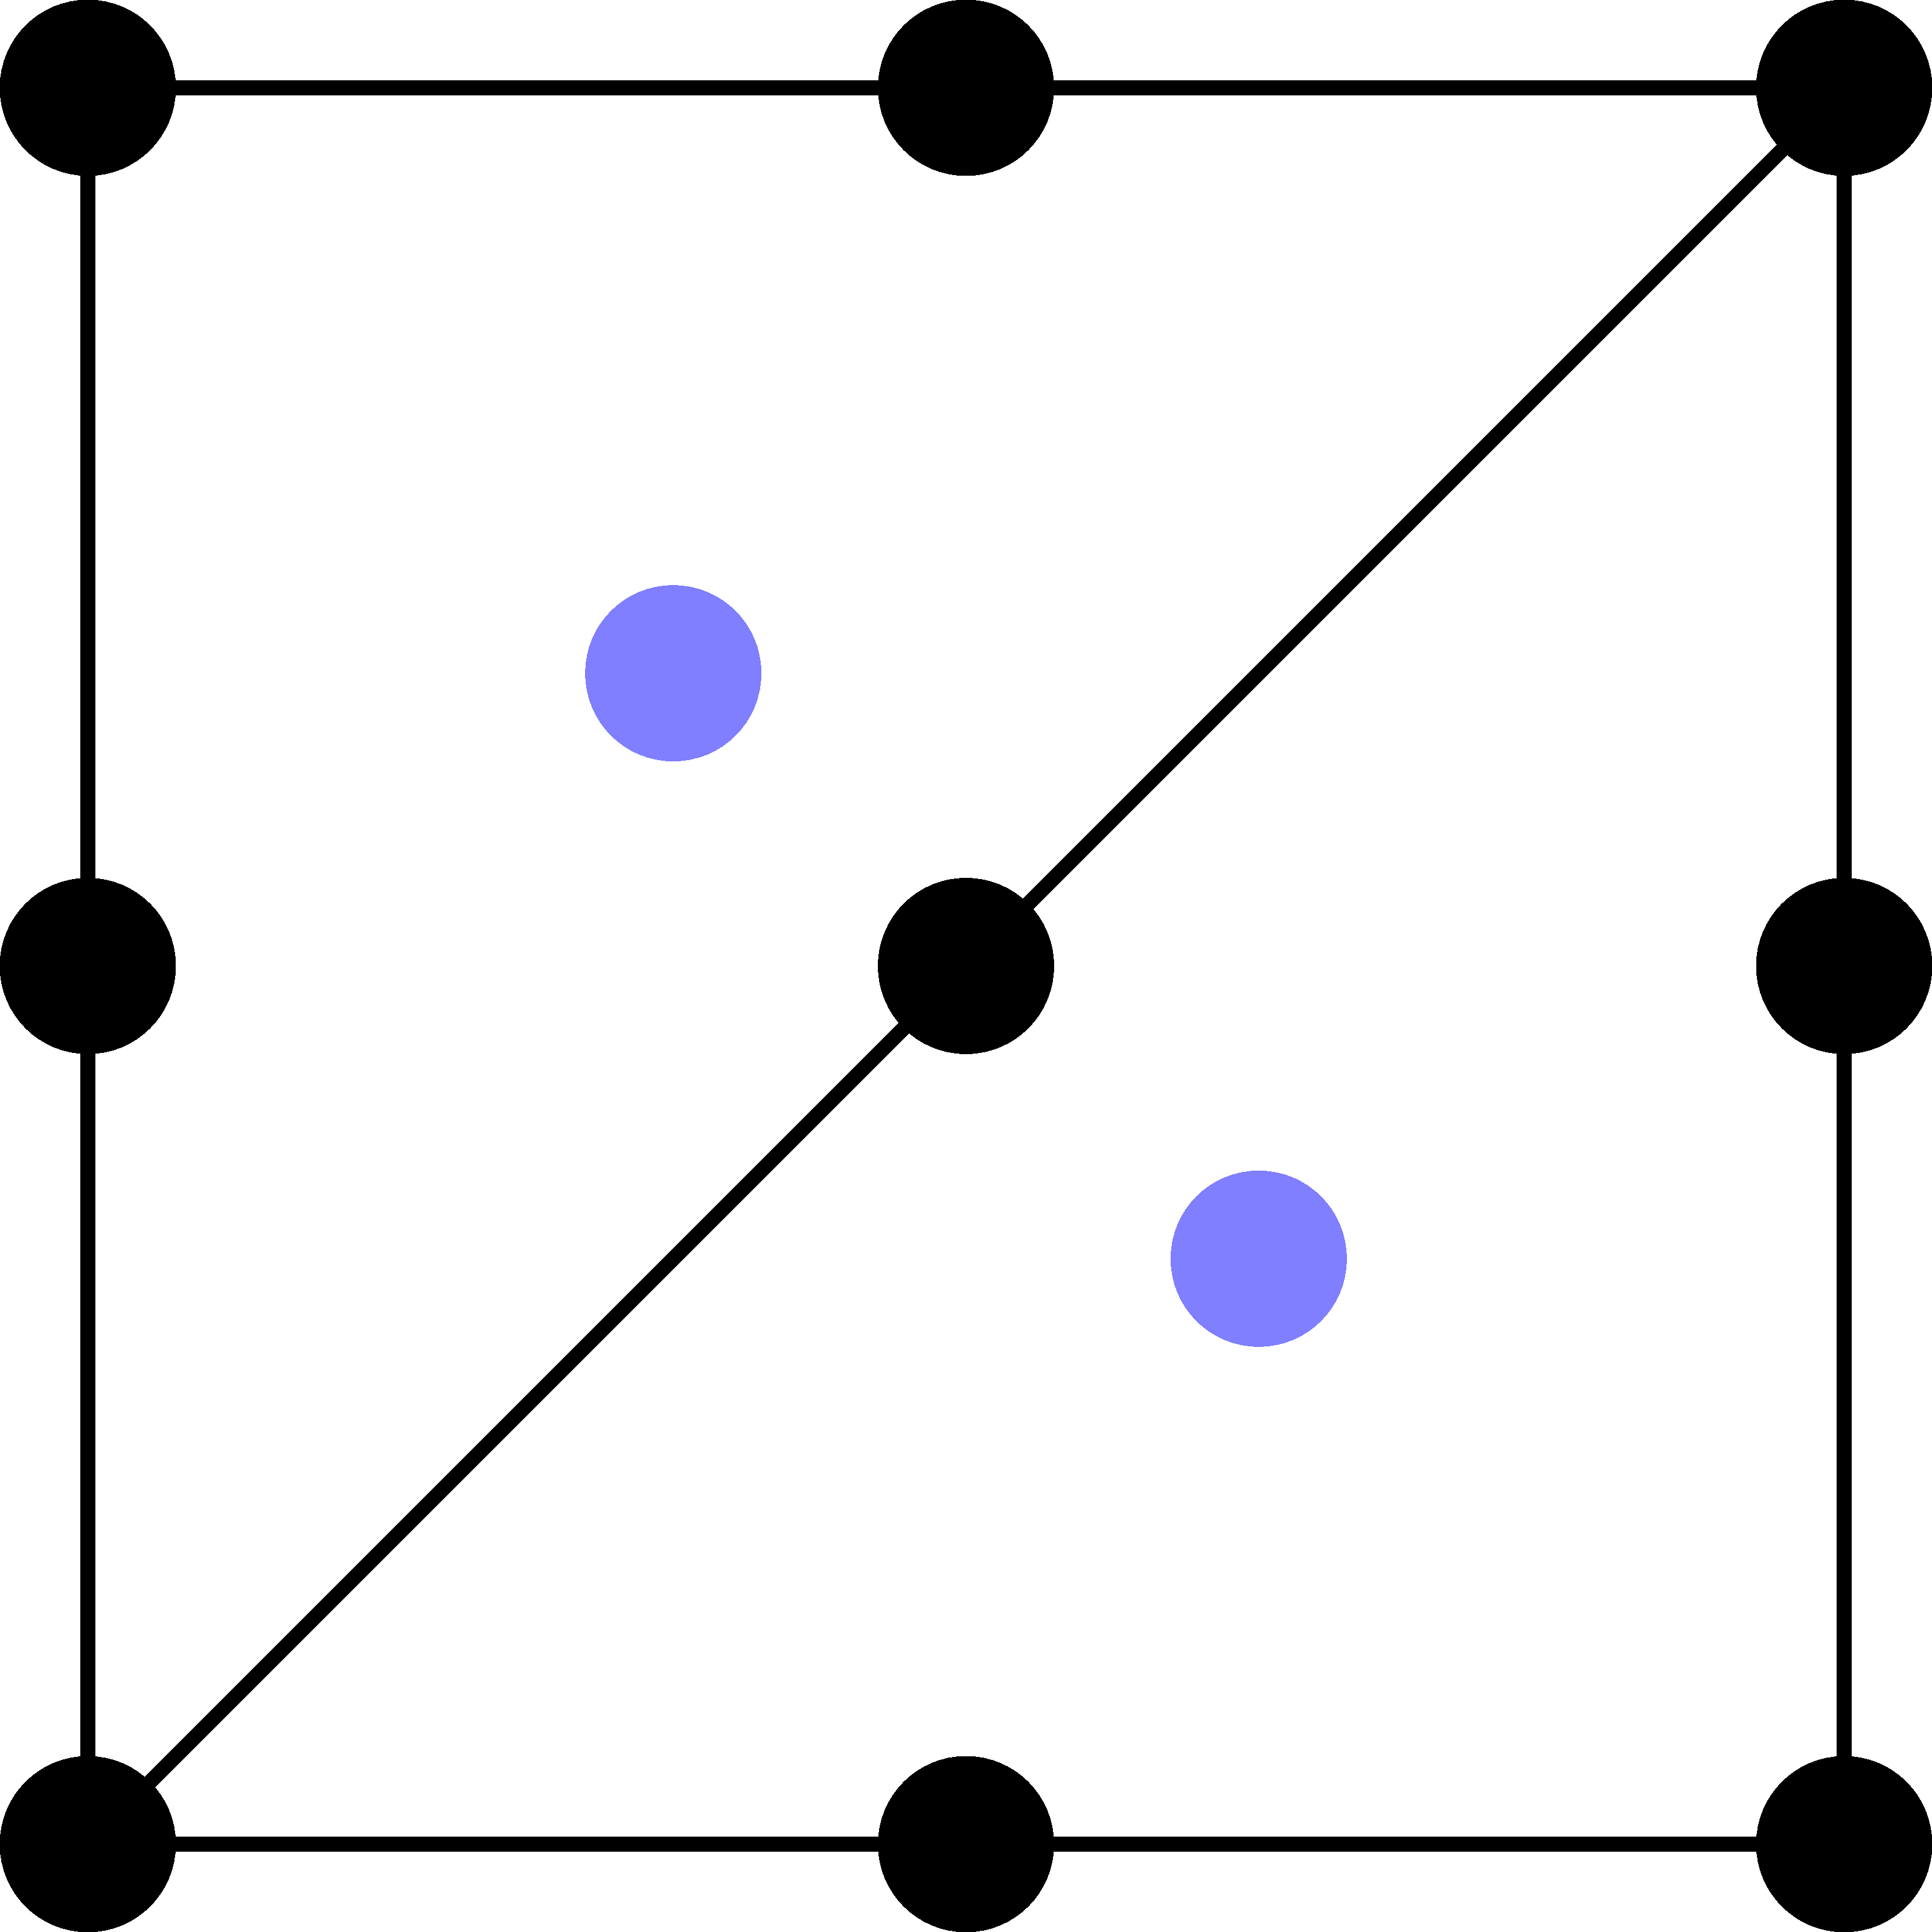
\includegraphics[width=0.9\textwidth]{figures/CrouzeixRaviart.png}
            \end{minipage}\\Crouzeix-Raviart element \cite{crouzeix1973}
        \end{tabular}
        &4&\checkmark & & \checkmark\\
        \hline
        \multicolumn{5}{c}{
                \begin{tabular}{c@{\hspace{24pt}}c}
                    \raisebox{-0.2\height}{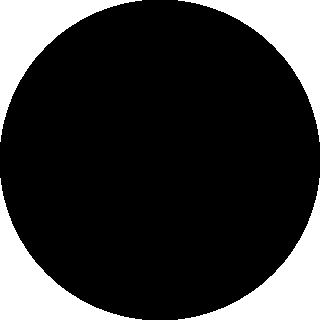
\includegraphics[width=10pt]{figures/legend_u.png}} :位移节点 &
                    \raisebox{-0.2\height}{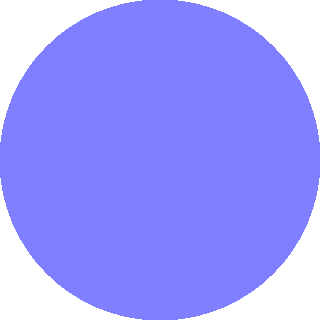
\includegraphics[width=10pt]{figures/legend_p.png}} :压力节点 
                \end{tabular}}\\
        \hline
    \end{tabular}
\end{table}

值得注意的是,从上述T3P1单元与Q4P1单元例子可以观察到,即使将两个单元中的压力节点数设置为最小值1,其仍然无法满足LBB稳定性条件。这一现象主要源于传统有限元离散方案中节点布置方式的固有局限性:在传统有限元混合离散方案中,压力节点必须依附于单元进行布置,且每个单元至少需要布置一个压力节点,这种限制导致节点数量无法根据位移节点与压力节点的最优比例需求进行灵活调整。因此,在传统有限元混合离散方案框架下,无论是三角形3位移节点单元还是四边形4位移节点单元,均不能满足LBB稳定性条件。

\section{小结}
本章从泛函分析的角度出发,再次验证了LBB稳定性系数是主应力刚度矩阵与偏应力刚度矩阵的广义特征值的平方根。
随后,通过引入适定的完备多项式空间,对LBB稳定性系数的估计式进行了进一步化简,从而建立了一个新的LBB稳定系数估计表达式。
在这一过程中,将LBB稳定系数表达式中的空间维度与位移和压力的自由度个数联系起来,即与体积约束比建立联系。
通过对二维和三维空间中位移和压力自由度的详细讨论,总结出了最优约束比的取值范围。
利用这一新的估计表达式,对已有的二维和三维情况下有限元离散算法进行了验证,并将结果与数值验证结果和解析证明结果进行对比,初步证明了所提方法的可行性。
